\chapter{Results and Discussion for ACL and HOL Verification}
\label{cha:results-disc-acl}

\section{State Machines and Secure State Machines: Transition Types and Principals}
\label{sec:state-mach-secure}



What distinguished a state machine from a \emph{secure} state machine was the addition of transition states and principals.  The "non-secure" state machine was defined by the allowable states and commands (inputs).  This state machine was modified to produce a \emph{secure} state machine by imposing restrictions on whether or not a state machine could change states. These restrictions were expressed as transition types and \emph{which} transition type was applied to the state machine was determined by the security context.  The transition types \emph{exec}, \emph{trap}, and \emph{discard} determined whether a command was allowed to be executed, trapped, or discarded, respectively.  Because HOL is a strongly-typed language, we also needed one more type called an option type.  The option type allowed us to return \emph{SOME} command or indicate that there was \emph{NONE}.  When combined, commands in a secure state machine took one of three forms: \emph{exec (SOME cmd), trap (SOME cmd)}, or \emph{discard (SOME cmd)}.  \emph{exec (SOME cmd)} was executed.  \emph{trap (SOME cmd)} and \emph{discard (SOME cmd)} were not.  In addition, \emph{trap (SOME cmd)} was reduced to \emph{trap NONE} in some of the theorems.  This reduction effectively nullified the command \emph{cmd} (because trapped commands were not executed).\\
  
Trapped commands were not necessary for our project.  Trapped commands had a specific function in the virtual machine world for which the original parameterizable \emph{secure} state machine ssm11 was implemented.  In our project, trapped commands were discussed as feedback mechanisms such as informing the \emph{secure} state machine that "an unauthorized person made a request."  But, we did not prove any theorems regarding them at the time of this documentation.  Discard commands were handled similarly.  Both trapped and discarded transition types were described in the next state and next output functions (described below) because they were needed to use ssm11 and ssm.  \\
  
In a \emph{secure} state machine, principals issued commands.  Principals were defined as entities (human or non-human) that made request (gave orders) for a state machine to change states.  Principals making requests needed to be authenticated and authorized on the requests before the requests were honored.  In general, authentication could be verified by ID badge, password, thumb print, etc., or any combination of these.  Authentication for our \emph{secure} state machines was governed by our interpretation of the patrol base operations.  We assumed that familiarity amongst the soldiers was sufficient to authenticate individuals and no cryptographic methods were needed.  For our \emph{secure} state machines, authentication was verified by the authenticationTest function. The authenticationTest function defined which principals were authenticated for \emph{which} set of commands.\\
  
Authorization, on the other hand, defined which commands a known principal was authorized to issue.  To distinguish authorization from authentication, think of authentication as "who are you?" and authorization as "what are you allowed to do?"  In general, authorization is defined by an organization's policies and/or security context. For our patrol base operations, it was sufficient to authorize one or two principals to issue commands to change states.  These principals and their authority were contained in a security context list.  For our project, these lists consisted of statements of the form "some principal has authority over some set of commands."  In the ACL, that same statement was of the form "Platoon Leader controls someSetOfCommands." \\
  
The authentication and authorization of principals for our \emph{secure} state machines followed the HOLReports of least privilege.  This principle stated that privilege be given to the least number of principals (or entities) necessary to accomplish the goal.   Thus, in our \emph{secure} state machines, only one or two principals were authorized to issue commands.   



\section{Next State and Next Output Functions}
\label{sec:next-state-next}



In general, state machines were defined by their states, inputs, and outputs.  For our state machines, we called inputs "commands".  State machines were described with diagrams for human consumption, whereas the next state and next output functions were required by HOL.  The next state functions described an initial state, a command, and the state that followed if the command was executed.  The \emph{secure} state machines required the addition of the transition types described above.  Thus, these next state functions described an initial state, a transition type applied to a command, and the next state.  The next state function for an example \emph{secure} state machine was shown in the text box below.\\
  
  \begin{figure}[h]
  \centering
  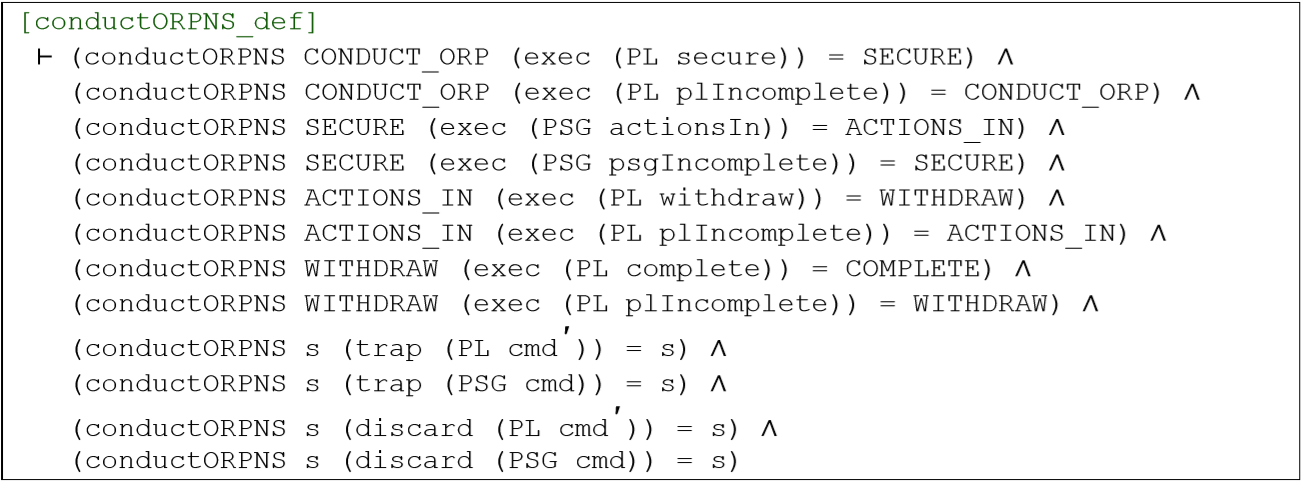
\includegraphics[width=0.8\linewidth]{conductORPNS.PNG}
\end{figure}

In the line \emph{CONDUCT_ORP (exec (PL secure)) = SECURE)}, \emph{CONDUCT_ORP} was the initial state, \emph{(exec (PL secure))} was the transition type applied to the command secure, and SECURE was the state of the secure state machine if the command was executed.  In the line, \emph{s (trap (PL cmd′)) = s}, \emph{s} was a variable for any valid state, \emph{(trap (PL cmd))} was the transition type applied to the command \emph{cmd}, and \emph{s} was the state after the trap command was applied.  Note that trapped transitions were not allowed and the state machine did not change states.  The \emph{discard} transition type followed a similar logic.  \emph{PL} and \emph{PSG} were constructors that helped HOL determine what type of command followed. \emph{PL} indicated that the command was a Platoon Leader command \emph{(plcommand)} and \emph{PSG} indicated that the command was a Platoon Sergeant command \emph{(psgCommand)}.  \\
  
Next output functions followed a similar logic.  Although, we did not focus on outputs for our secure state machines, they were required to parameterize ssm11 and ssm.  The next output function for the \emph{secure} state machines described an initial state, a transition type applied to a command, and the output that resulted.  Compare this to the next state function by replacing the final states in the example above with the output in the example below.  (Note that outputs begin with a capital letter and contained both capital and lowercase letters whereas the states are all capital letters.)  Everything else is the same.    The next output function for the same \emph{secure} state machine described above was shown in the text box below.   The pattern should be evident.\\
  
  \begin{figure}[h]
  \centering
  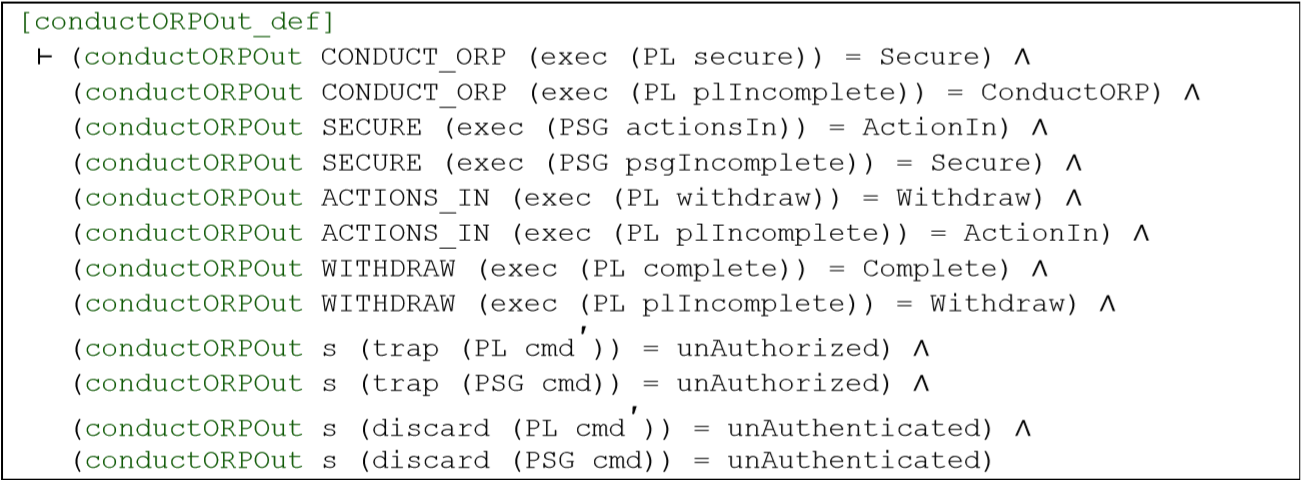
\includegraphics[width=0.8\linewidth]{conductORPOut.PNG}
\end{figure}


\subsection{states, commands/inputs, outputs, and Principals}
\label{sec:stat-comm-outp}

 The basic datatypes were defined for all theories in the OMNIType Theory (defined in HOL/OMNITypeScrip.sml).  These were \emph{state}, \emph{command}, \emph{output}, and \emph{principal}.   In their definitions, each of these contained a constructor followed by a state-level defined datatype.   An example of the \emph{command} datatype definition in the OMNIType Theory was shown below.\\
  
  \begin{figure}[h]
  \centering
  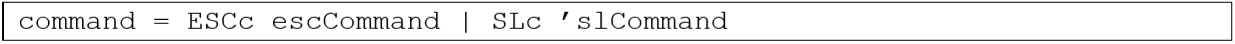
\includegraphics[width=0.8\linewidth]{command.PNG}
\end{figure}

  \emph{SLc} was the constructor for a command of type \emph{slCommand} (state-level command).  These commands were to be defined at the state-level secure state machines. \emph{ESCc} was the constructor for the  \emph{escCommand} (escape-command).  The escape states and commands were designed to allow abortion of the operation.  The idea was that certain conditions, such as contact with enemy, required escape from any state.  These states were not verified in HOL, but they were retained in the OMNIType Theory for future work. \\
  
   The other OMNIType datatypes were shown below.  They follow a similar logic and nomenclature. \\
  
  \begin{figure}[h]
  \centering
  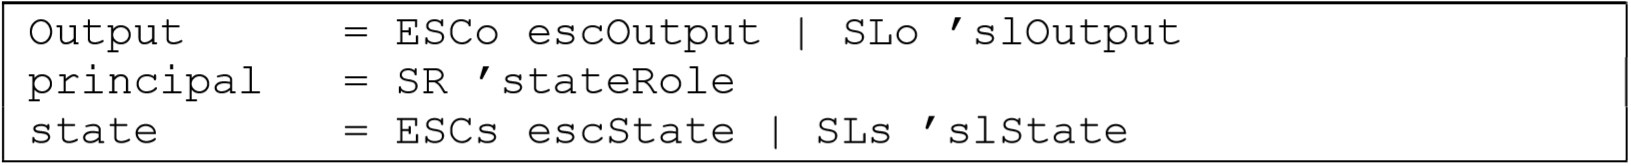
\includegraphics[width=0.65\linewidth]{output.PNG}
\end{figure}

  In the \emph{secure} state machines, \emph{command, state, output}, and \emph{principal} were defined with the specific commands for that state.  For example, the text box below shows the definition of these datatypes for a secure state machine that used only one principal. \\\\\\\\\\\\\\\\\\\\\\\\\\\\\\
  \begin{figure}[h]
  \centering
  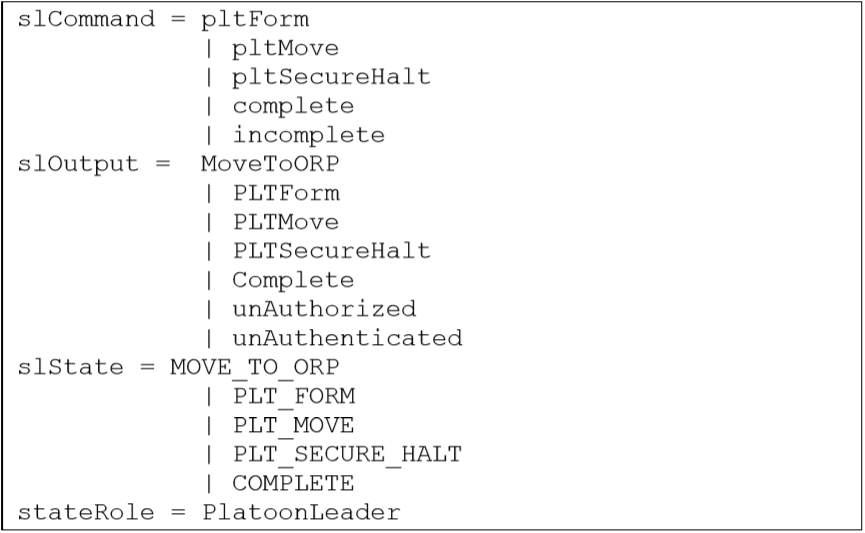
\includegraphics[width=0.6\linewidth]{slCommand.PNG}
\end{figure}

  For \emph{secure} state machines with multiple principals, it was easier to define commands that each principal could issue separately from one another.  Therefore, the Platoon Leader could make Platoon Leader commands \emph{(plCommand)} and the Platoon Sergeants could make Platoon Sergeant commands \emph{(psgCommand)}.  \emph{stateRole, slOutput}, and \emph{slState} did not require separate commands.  An example of these datatype definitions for \emph{slCommand} was shown below.  
  
  \begin{figure}[h]
  \centering
  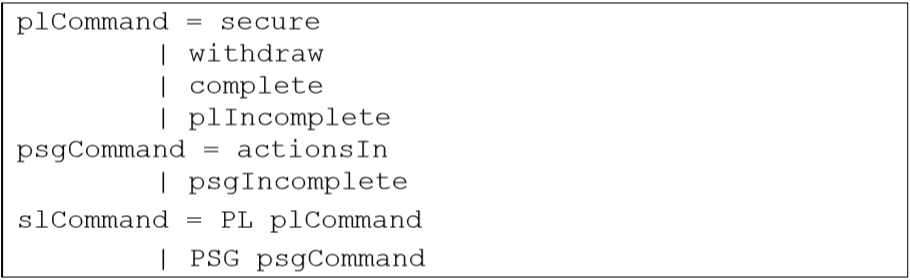
\includegraphics[width=0.6\linewidth]{plCommand.PNG}
\end{figure}



\section{Configurations}
\label{sec:configurations}

State machines were defined by their next state and next output functions.  But, \emph{secure} state machines also required principals, authentication, and authorization.  In addition, to the next state and next output functions, our \emph{secure} state machines were defined by configurations.  These configurations included the following entities:
\begin{itemize}
\item Authentication Test Function
\item State Interpretation Function
\item Security Context List
\item Input
\item Current State
\item Output\\
  \end{itemize}
  
\subsection{Authentication Test Function}
\label{sec:auth-test-funct}

This function tests the principals for proper authentication.  As described above, authentication for this project was assumed to be done by familiarity.  Thus, the authentication test function returned true if the authentication was verified and false otherwise.  
  
\subsection{State Interpretation Function (state specific rules)}
\label{sec:state-interpr-funct}

The state interpretation function defined logical rules that were specific to each state.  For our project, the state interpretation function was not used.  However, it was required for the configurations.  Thus, \emph{stateInterp} function was defined to return the trivial value TT, the ACL logical value for true.  
  
\subsection{Security Context List}
\label{sec:secur-cont-list}

The security context consisted of the policies regarding \emph{which} principal had authority to make \emph{which} commands. The security context was thus a list of ACL formulas of the form "SomePrincipal controls someCommand", where \emph{controls} is the ACL logical expression of authority.
  
\subsection{Input}
\label{sec:input}
The input was of the form "somePrincipal says someCommand."  \emph{says} is the ACL logical expression of a request.   In this case, somePrincipal is requesting to execute someCommand.  In ssm11, the input was a single ACL \emph{says} statement.  In the ssm, the input was a list of these statements, i.e.,  ["somePrincipal1 says someCommand1", "somePrincipal2 says someCommand2", ...].\\
    
In the configurations and the theorems, the input was represented as an input stream.  The input stream was expressed in HOL as a list.  The list was of the form firstElement::remainderOfList.  The "::" is the "cons" operator in HOL and it separated the first list element from the remainder of the list.  The first element of the list was the ACL request, i.e., "somePrincipal says someCommand" in the case of ssm11 and the corresponding list in the case of ssm.   That is, the input for ssm11 was a list and for ssm was a list of lists.  The remainder of the list was simply a variable for our theorems.  This variable was typically named \emph{ins}.  Thus, an input in our configurations had the following form.\\
    
    \begin{figure}[h]
  \centering
  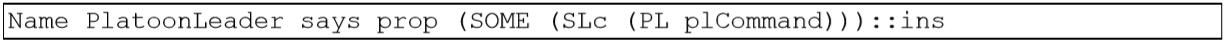
\includegraphics[width=0.8\linewidth]{name.PNG}
\end{figure}

The left side of the "::" operator was the strongly-typed version of "somePrincipal says someCommand." The right side was the variable ins.  \emph{Name} was the ACL constructor for a principal.  The principal in this example was \emph{PlatoonLeader}.  prop was the ACL constructor for a proposition.  In our example, propositions were commands.  \emph{SOME} told HOL that what follows was some command (rather than NONE).

\subsection{Current State}
\label{sec:current-state}

The current state was the current state.  Nothing too complicated here.

\subsection{Output}
\label{sec:output}

Outputs were not used, but were defined in order to use ssm11 and ssm.  They were often represented with the variable out, outs, or output.  Outputs in configurations were also streams.  After a transition from one state to another was executed (or trapped or discarded), the resulting output was "cons"ed onto the previous output stream.  This looked like \emph{newOutput::outputStream}.

\section{Theorems}
\label{sec:theorems}

For this project, there was one primary theorem.  It proved that a transition was executed if and only if the proper authentication and authorization were verified.  This was sufficient to satisfy the principle of complete mediation.  It was proved for each principal issuing commands.  Thus, for secure state machines with two principal, one theorem was proved for each principal.  An example of this theorem was shown below.\\
  
\begin{figure}[h]
  \centering
  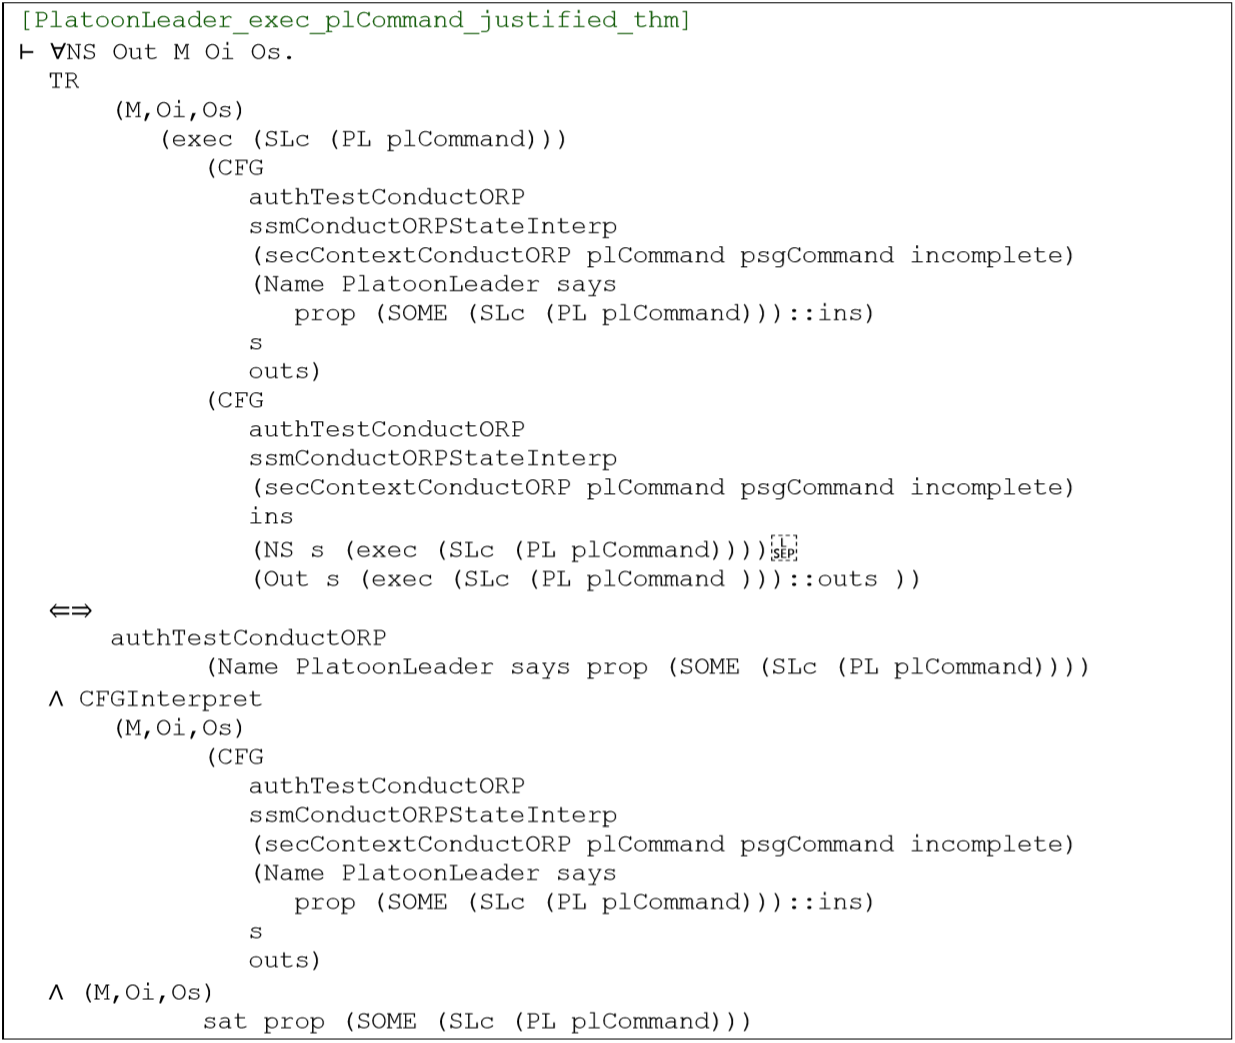
\includegraphics[width=0.8\linewidth]{PlatoonLeader.PNG}
\end{figure}

The name of this theorem was \emph{PlatoonLeader_exec_plCommand_justified_thm}.  The theorem justified executing transitions wherein the \emph{PlatoonLeader} issued commands of type \emph{plCommand}.  The next line stated that this theorem was valid for all next state (NS) functions, output (Out), and Kripke Structures\footnote{Kripke Structures are explained in the text book \emph{Access Control, Security, and Trust: A Logical Approach}. Kripke Structures were not defined for the patrol base operations.  But, they are part of the ACL and are required for application of the ACL theories.} (M, Oi, Os).  \\

\emph{TR} was the Transition Relation function.  It took as input a Kripke Structure, a transition type with a command, and an initial configuration.  It returned a final configuration.  In this example, the transition type with the commands \emph{(exec (SLc (PL plCommand)))} told HOL that the transition from the initial to final state was executed for commands of type \emph{plCommand}.   \\
  
 The initial configuration was preceded by the constructor \emph{CFG}.  The authentication test function was named \emph{authTestConductORP}.  The state interpretation function was named \emph{ssmConductORPStateInterp}.  The security context list was named \emph{secContextConductORP}.  This took three parameters: \emph{plCommand}, \emph{psgCommand} and \emph{incomplete}.  These were the allowable command datatypes.  The input stream was Name \emph{PlatoonLeader says prop (SOME (SLc (PL plCommand)))::ins}. The first element of this stream (before the "::" cons operator) was the ACL request to change states.  The other part of the input stream was the variable \emph{ins}.  The current state was \emph{s}.  The output was \emph{outs}.  \\
  
 The final configuration was also preceded with the constructor CFG.  In this final configuration, the first three elements \emph{authTestConductORP}, \emph{ssmConductORPStateInterp}, and \emph{secContextConductORP} were unchanged.  The input stream changed by pealing-off the first element.  ins remained.  The state changed by applying the next state \emph{(NS)} function.  The function call was \emph{(NS s exec (SOME (SLc (PL plCommand)))}.  Similarly, the output changed by adding the initial output to the output stream at the front of the list: \emph{(OUT s exec (SOME (SLc (PL plCommand)))::outs)}.  \\
  
In summary, this first part of the biconditional stated that the result of executing the command \emph{plCommand} with the transition type \emph{exec} was a transition from the initial configuration to the next configuration.\\
  
The second part of the biconditional checked the authorization and authentication of the principal issuing the request.  It was a conjunction of three parts.  For the first part, the \emph{authTestConductORP} had one parameter, the input request \emph{Name PlatoonLeader says prop (SOME (SLc (PL plCommand)))}.  \emph{authTestConductORP} returned true if \emph{PlatoonLeader} was authenticated on \emph{plCommands} and returned false otherwise.  \\

The second part, \emph{CFGInterpret} essentially joined the elements in the configuration to make it easier for HOL to work with.  It took two parameters, a Kripke structure and the initial configuration.  It returned a conjunction of elements from the initial configuration.  Those elements were the security context, the input, and the state interpretation function applied to the state.  Unlike the first part, this part did not return a boolean value of true or false.\\
  
The third part verified that the command/proposition \emph{prop (SOME (SLc (PL plCommand))} satisfied the Kripke structure.  This meant that the command was justified. \\
 
In summary, the first and last part of the biconditional proved that the transition from initial state to final state was executed if and only if the \emph{PlatoonLeader} issued a \emph{plCommand} and the \emph{PlatoonLeader} was authorized on the \emph{plCommand}.  \\
  
HOL was used to prove \emph{PlatoonLeader_exec_plCommand_justified_thm}.  To prove this theorem, we parameterized an ssm11 theorem named \emph{TR_exec_cmd_rule}.  The \emph{TR_exec_cmd_rule} was used with the ISPECL rule in HOL to replace the variables in \emph{TR_exec_cmd_rule} with the variables used in \emph{PlatoonLeader_exec_plCommand_justified_thm}.  An example of the ISPECL rule used to prove \emph{PlatoonLeader_exec_plCommand_justified_thm} was shown below.\\
  
  \begin{figure}[h]
  \centering
  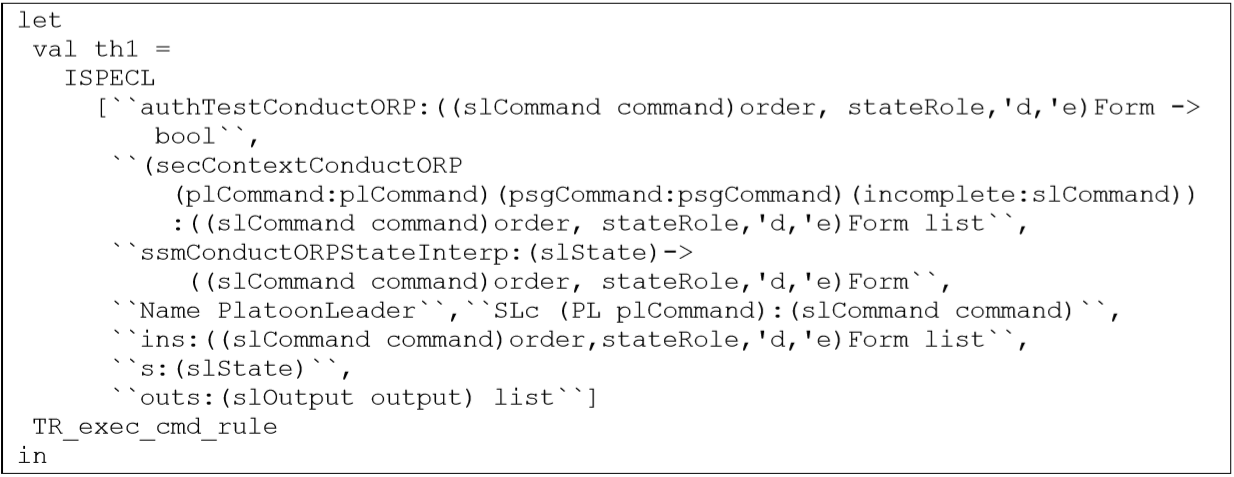
\includegraphics[width=0.8\linewidth]{th1.PNG}
\end{figure}

HOL needed the double back-quotes `` to recognize terms.  The excess "junk" that followed each variable (or parameter) was the typing.  Remember HOL was a strongly-typed language.  Thus, the first parameter was \emph{authTestConductORP}.  The second was \emph{secContextConductORP}. The third was the HOLReports \emph{Name PlatoonLeader}.  The fourth parameter was the command \emph{SLc (PL plCommand)}.  The fifth was the input stream (without the first element) \emph{ins}.  The sixth was the state \emph{s}.  The seventh was the output stream outs.  The \emph{let} and \emph{in} statements were part of the proof construct.  \emph{val th1 =} essentially set-up this specialized version of \emph{TR_exec_cmd_rule} and temporarily saved it as \emph{th1}.   \\

To prove \emph{PlatoonLeader_exec_plCommand_justified_thm} we needed one more theorem, actually a lemma.  This lemma proved the second and third part of the second half of the biconditional.  It was shown below.\\
  
  \begin{figure}[h]
  \centering
  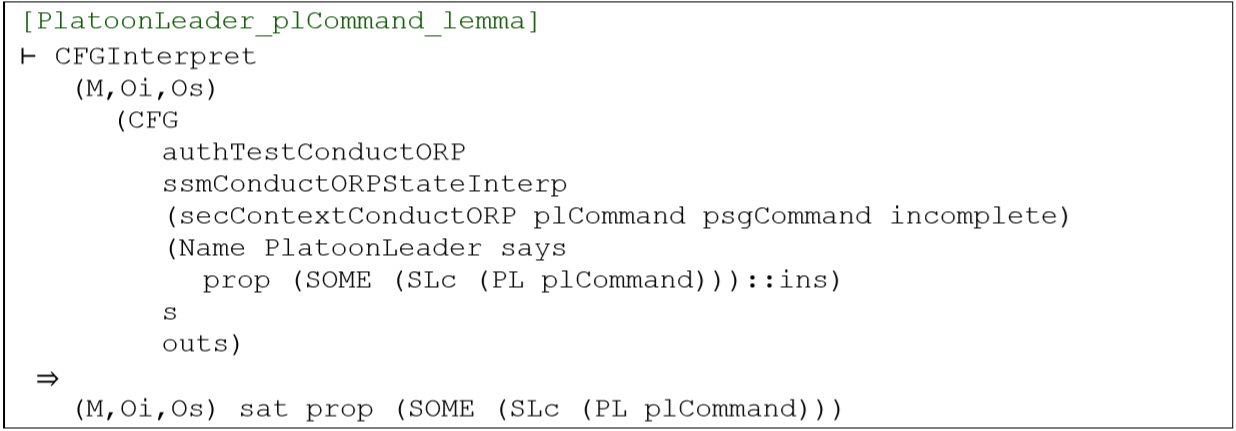
\includegraphics[width=0.8\linewidth]{PlatoonLeader2.PNG}
\end{figure}

\emph{PlatoonLeader_plCommand_lemma} proved that the initial configuration justified the proposition \emph{(SOME (SLc (PL plCommand)))}.  To convince HOL the lemma was true, we directed HOL to look at several definitions: the \emph{authTestConductORP}, which stated that the \emph{PlatoonLeader} was authenticated on the input; the \emph{ssmConductORPStateInterp}, which was defaulted to TT (ACL for true); and the \emph{secContextConductORP}, which stated that \emph{PlatoonLeader} controls the input.  With this information reformatted by the \emph{CFGInterpret} function, HOL used the following ACL rule to justify the proposition.\\
  
  \begin{figure}[h]
  \centering
  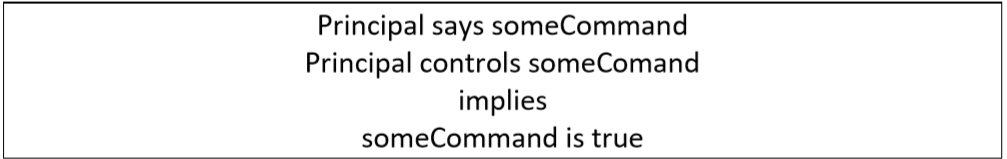
\includegraphics[width=0.6\linewidth]{principal.PNG}
\end{figure}



\section{Parameterizable Secure State Machines}
\label{sec:param-secure-state}


\subsection{ssm11}
\label{sec:ssm11-1}

ssm11 was the initial \emph{secure} state machine that was verified before the start of this project.  The name means "secure state machine version 1.1".  The original version was ssm1.  ssm1 was modified for this project.  The modifications were minor.  They included a change of name from \emph{inst} in the original to \emph{order} in ssm11.  Also, discard transitions were modified to act like the \emph{trap} transitions.  Although, neither \emph{trap} nor \emph{discard} were the focus of this project. \\
  
The reason ssm1 was used was because it represented a parameterizable \emph{secure} state machine theory that was already implemented in HOL and that had already been verified.  For example, \emph{TR_exec_cmd_rule} was already proved in ssm11.  This means that to prove equivalent theory in our \emph{secure} state machines was easy, requiring replacement of the parameters in \emph{TR_exec_cmd_rule} with the parameters in our \emph{secure} state machine.  \\
  
ssm11 worked for the more abstract \emph{secure} state machines.  But, it required a major overhaul to accommodate multiple input statements.  The overhauled version was named ssm because the overhaul was significant enough to warrant it replacing all future versions of ssm11 (and ssm1).  However, we did not replace versions of ssm11 in this project if they were verified before the overhaul.  Any future secure state machines would use the new ssm, such as sub-sub-level secure state machines (if time allowed).  We did apply the new ssm to the ssmPlanPB \emph{secure} state machine.  We called this new version ssmNewPlanPB.  The older version that used ssm11, ssmPlanPB, may have been removed from the project folders by the time this documentation was complete.\\
  
 The sections below clarified areas of the ssm11.\\

  
\subsubsection{Configurations}
\label{sec:configurations-1}

Configurations were defined in ssm11 and implemented in the state-level \emph{secure} state machines.  Configurations were described above.  

  
\subsubsection{CFGInterpret Function}
\label{sec:cfgint-funct}

\emph{CFGInterpret} condensed the configuration into a "satisfies" list that was valid for all \emph{(M, Oi, Os)}.  In ACL, "satisfies" meant that some rule was valid for all Kripke structures.  \emph{CFGInterpret} reduced the configuration to a list of satisfies structures that could be reasoned with by the ACL. The definition of \emph{CFGInterpret} was shown in the text box below.\\
  
  \begin{figure}[h]
  \centering
  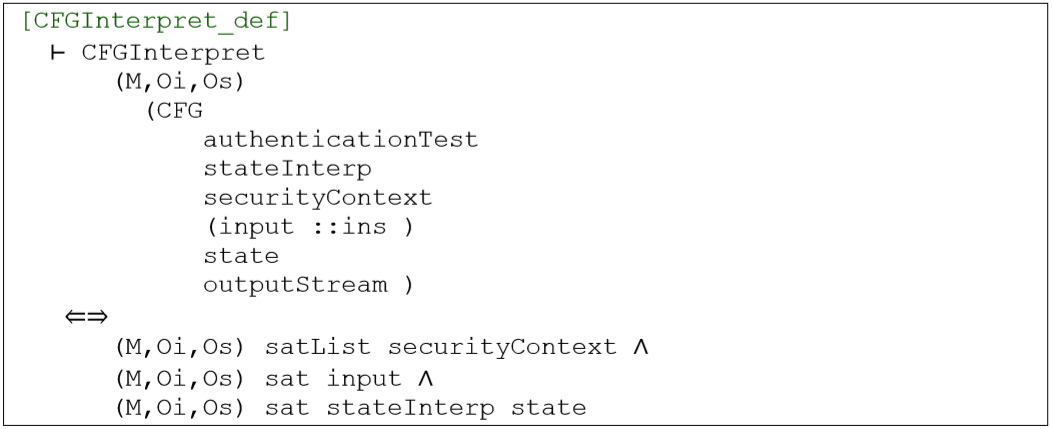
\includegraphics[width=0.8\linewidth]{CFGInterpret.PNG}
\end{figure}

 This was a biconditional.  The top part was the configuration.   The part following
  the $\Leftarrow \Rightarrow$ symbol was the "sat" statements that included the security context, the input,
  and the result of the state interpretation function applied to the state.


 \subsubsection{TR\textunderscore rules, TR\textunderscore cases, TR\textunderscore ind}
\label{sec:trtext-rules-trtext}


  \textit{TR_rules, TR_cases, TR_ind} described the \textit{secure} state machine \textit{TR}
  (Transition Relations).  The text box below showed the definition.  (Note that this definition
  looks different from many of the others in this document because this definition was taken from
  the ssm11Script.sml file whereas the others were taken from the EmitTeX generated pretty-printed files.)\\\\\\
  \\\\\\\\\\\\\\\\\\\\\\\\\\\\\\\\\\
  \begin{figure}[h!]
  \centering
  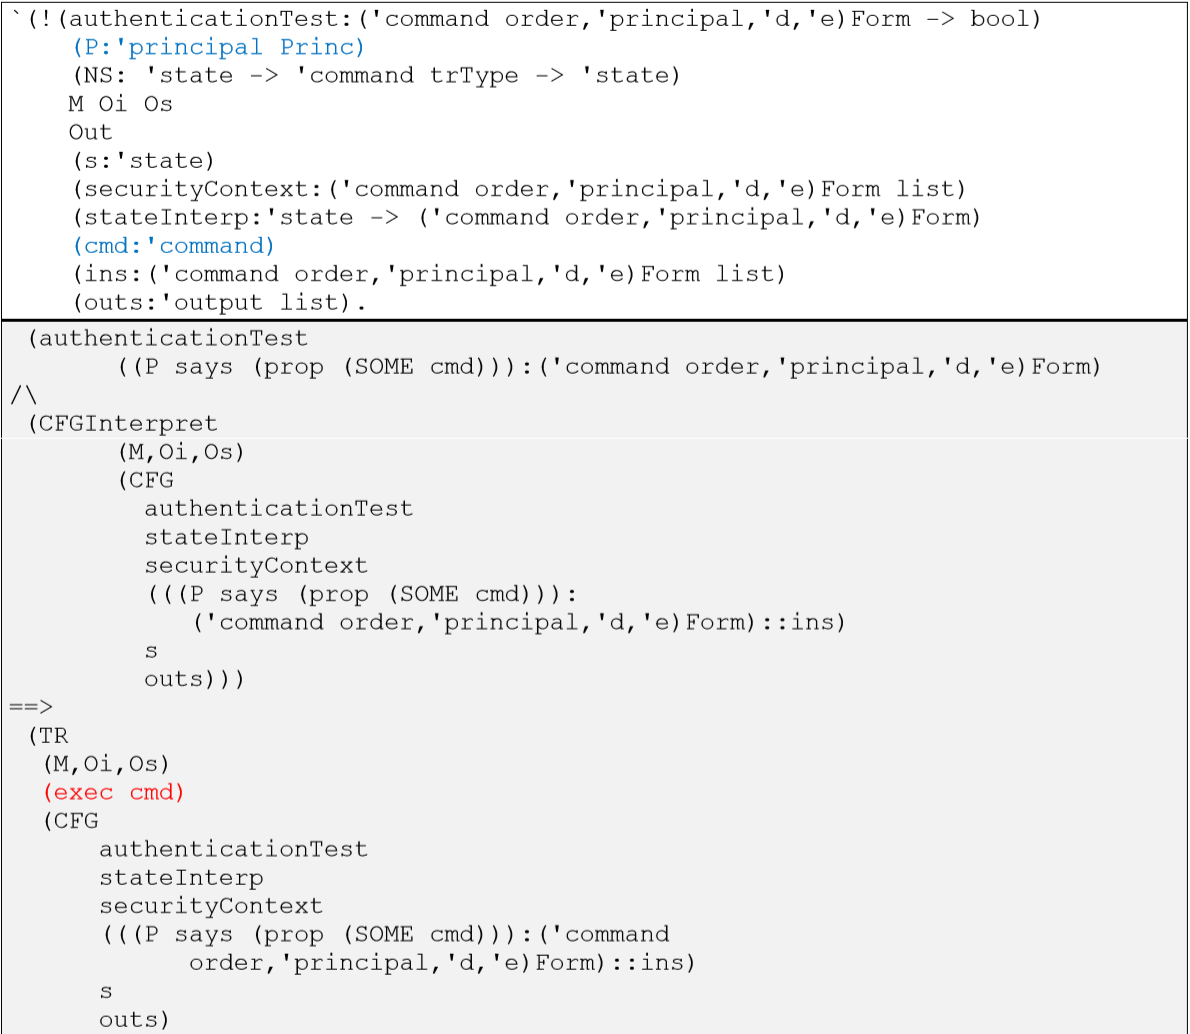
\includegraphics[width=0.8\linewidth]{TR1.PNG}
\end{figure}

\begin{figure}[h!]
  \centering
  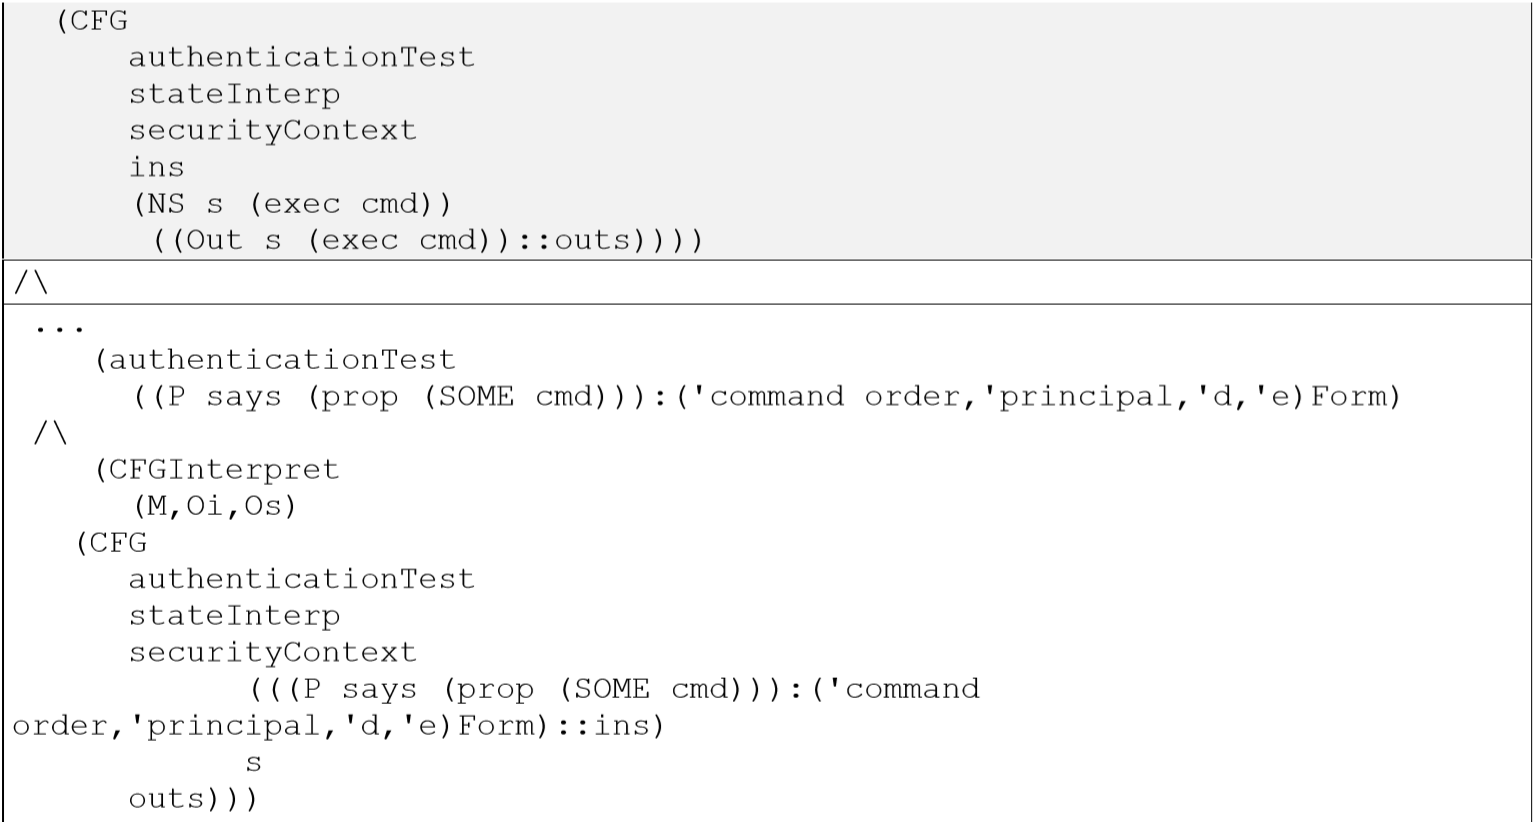
\includegraphics[width=0.8\linewidth]{TR2.PNG}
\end{figure}
\begin{figure}[h!]
  \centering
  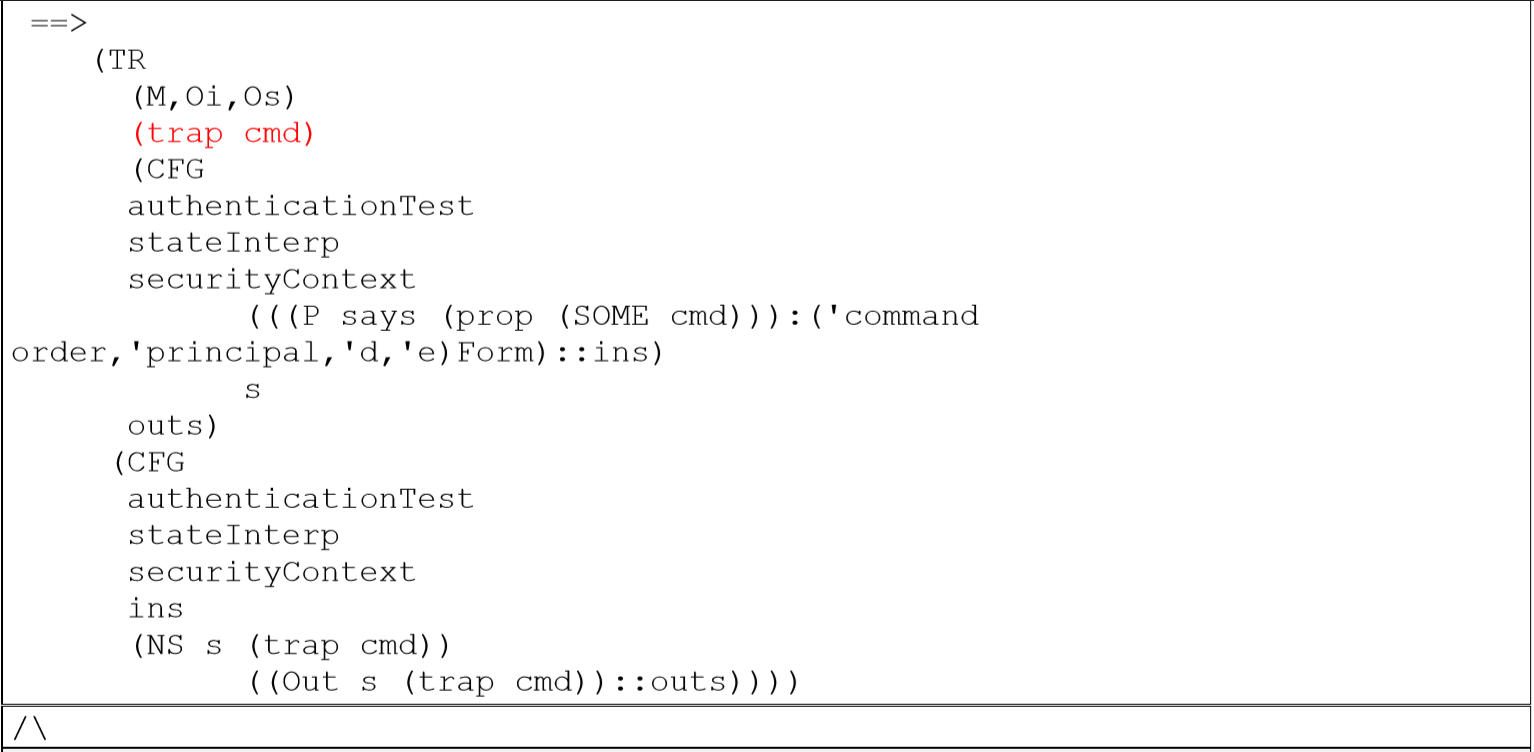
\includegraphics[width=0.8\linewidth]{TR3.PNG}
\end{figure}
\begin{figure}[h!]
  \centering
  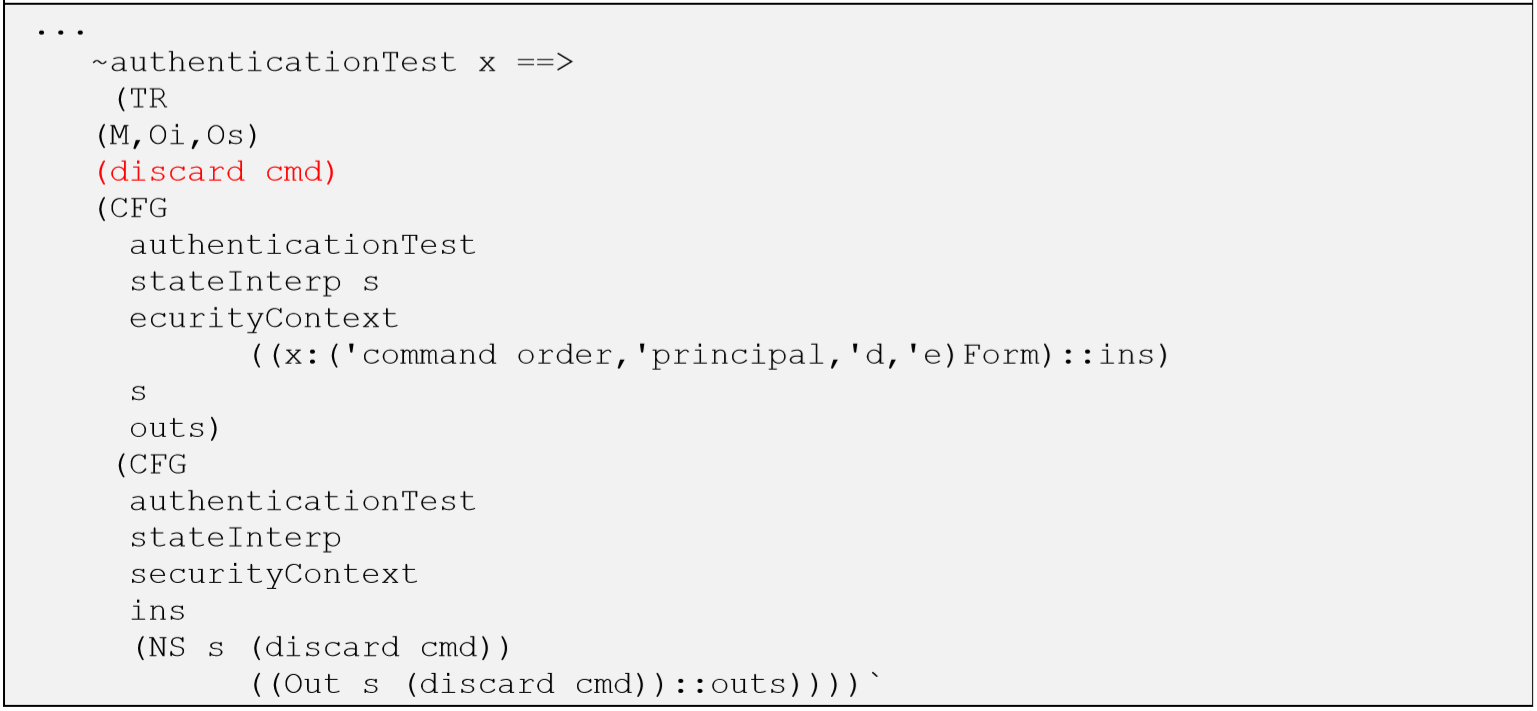
\includegraphics[width=0.8\linewidth]{TR4.PNG}
\end{figure}
 The above code was modified somewhat to make it easier to read in this document.
  The lines and highlighting distinguished logical sections of the code.  The top section
  stated that what followed was true for all the pertinent variables in the list.  This
  section was repeated two additional times in the code.  For brevity, it was repeated as "..."\\

 \sethlcolor{lightgray}
  
 The text in \textcolor{cyan}{blue} became problematic and prompted the overhaul of ssm11 to ssm.  This was discussed further in the appropriate section describing ssm.  The text in \textcolor{red}{red} were the transition types with the commands.  Notice that there was a separate transition type for each of the major blocks (save for the top block).  The blocks were also similar.  They described the rules for one transition type denoted in red. The first major block \hl{(lightly shaded)} described the Transition Relation for the exec transition type.  The second major block described the Transition Relation for the \emph{trap} translation type.  The last block described the Transition Relation for the \emph{discard} transition type.  The reader should have noticed the similarity of the definition above to \emph{PlatoonLeader_exec_plCommand_justified_thm} in the Theorems section.


\subsubsection{TR\textunderscore exec\textunderscore cmd\textunderscore rule}
\label{sec:trtext-exect-cmdt}


  \textit{TR_exec_cmd_rule} proved that a transition between states occurred if and only if
    the principal was authenticated and authorized on the executed command.  The theorem was shown below.\\
    
  \begin{figure}[h]
  \centering
  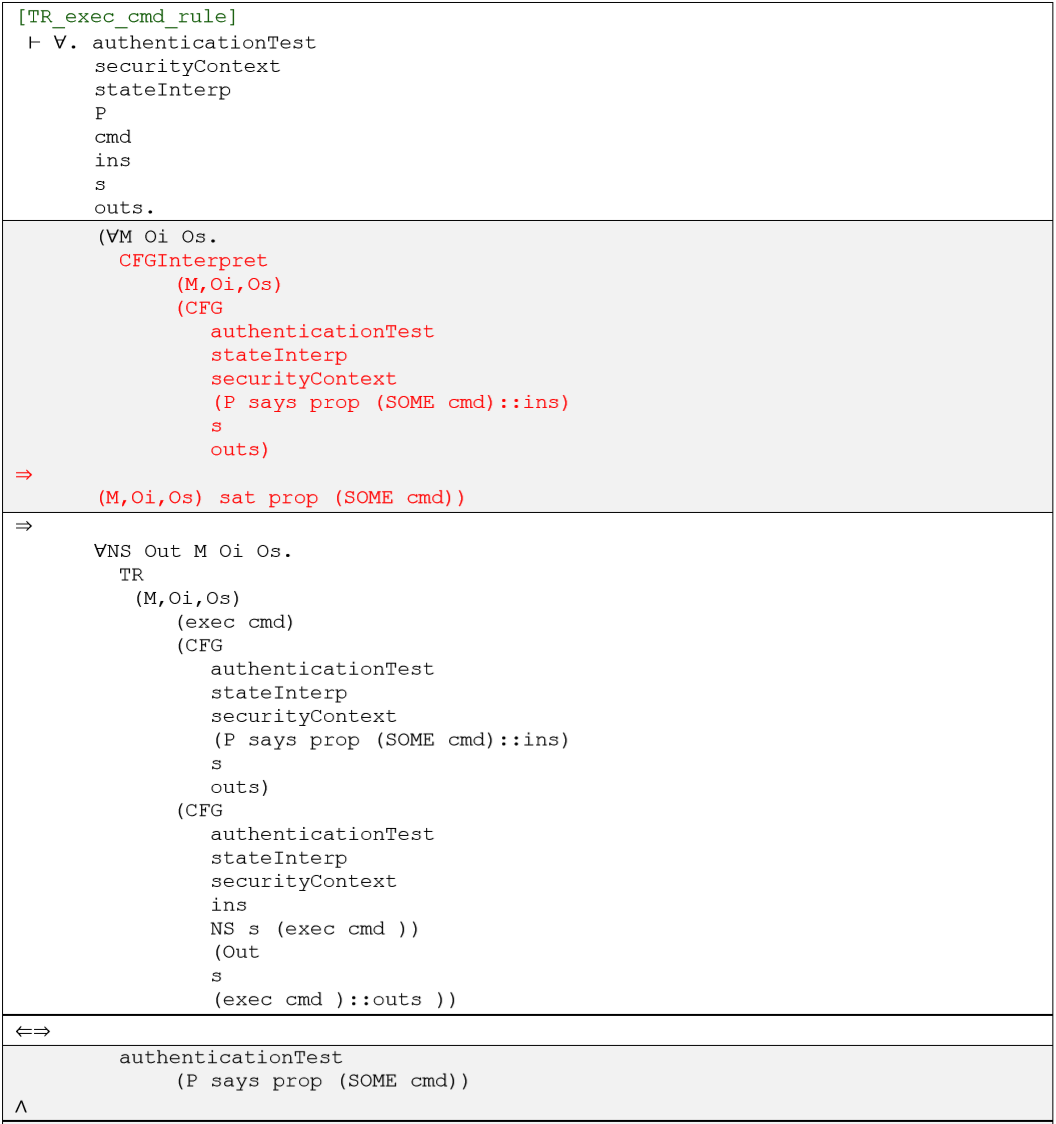
\includegraphics[width=0.8\linewidth]{TRexec.PNG}
\end{figure}
\begin{figure}[h!]
  \centering
  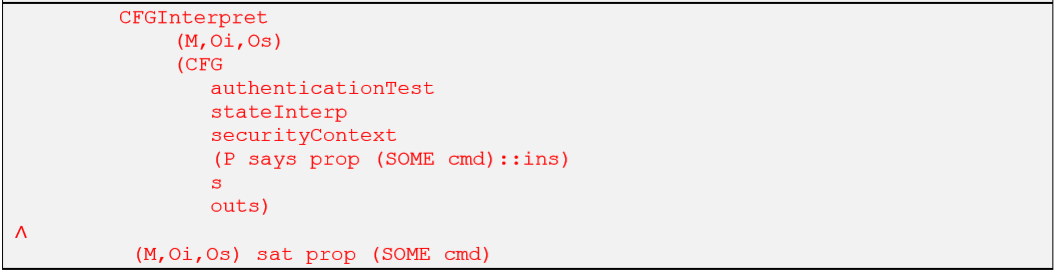
\includegraphics[width=0.8\linewidth]{TRexec2.PNG}
\end{figure}

Notice the greater similarity of this code to \emph{PlatoonLeader_exec_plCommand_justified_thm}.   That's because\emph{ PlatoonLeader_exec_plCommand_justified_thm} parameterized \emph{TR_exec_cmd_rule}.   The first part of this theorem was the "for all" list of parameters.  The red-text sections were essentially the parameterizable version of\emph{ PlatoonLeader_plCommand_lemma}.  They proved the principal was authorized and authenticated on the \emph{exec} transition type.  The non-highlighted text was the Transition Relations.  \\
  
\emph{TR_exec_cmd_rule, PlatoonLeader_exec_plCommand_justified_thm,} and \emph{PlatoonLeader_plCommand_lemma} are sufficiently similar that an expection of the code combined with the above description should have been sufficient to for the reader to understand.
 
 
\subsubsection{TR-trap-cmd-rule}
\label{sec:tr-trap-cmd}


\emph{TR_trap_cmd_rule} was similar to \emph{TR_exex_cmd_rule}.  There were two differences.  The first difference was that \emph{exec cmd} was replaced \emph{trap cmd}.  The second difference was that \emph{(M,Oi,Os) sat prop (SOME cmd)} was replaced with that \emph{(M,Oi,Os) sat prop  NONE}.  The highlighted code in the text box below showed this second difference.\\
  
  \begin{figure}[h]
  \centering
  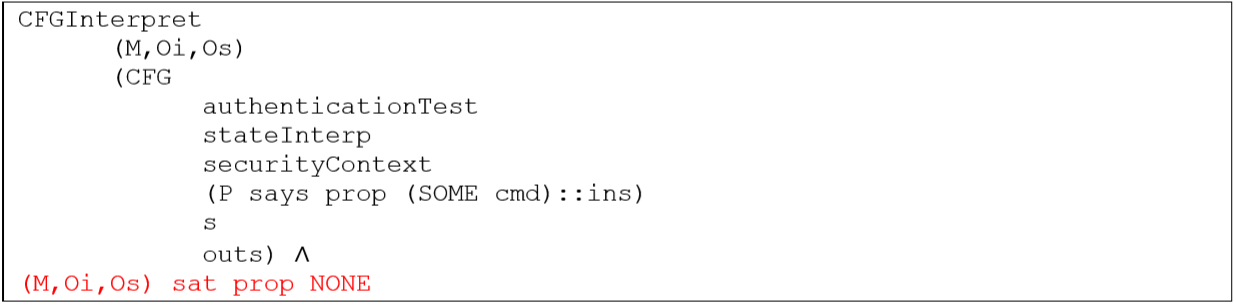
\includegraphics[width=0.75\linewidth]{CFGInterpret2.PNG}
\end{figure}


\subsubsection{TR-discard-cmd-rule}
\label{sec:tr-discard-cmd}

  \textit{TR_discard_cmd_rule} proved that the \textit{discard cmd} was applied to the state machine
  if and only if the authentication test failed.  (\textit{~authentication x}).  That code was shown below.\\
  
  \begin{figure}[h]
  \centering
  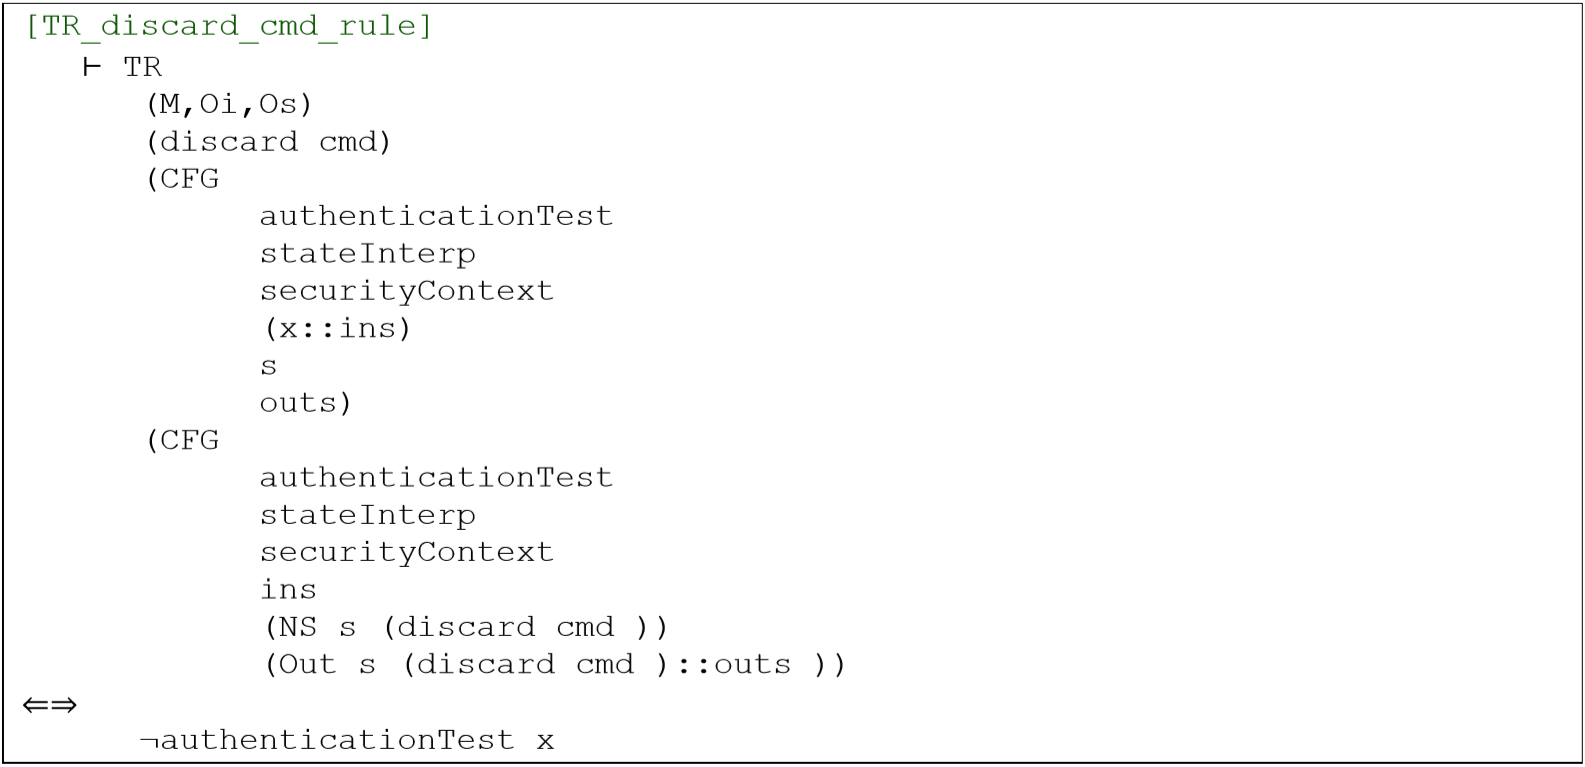
\includegraphics[width=0.75\linewidth]{TRdiscard.PNG}
\end{figure}

Other theorems and datatypes in the ssm11 supported the main theorems and datatypes described above.  The complete list of the theorems was shown in the EmitTeX pretty-printed code in the appendix.


\subsection{ssm}
\label{sec:ssm-1}

ssm was an overhaul of ssm1.  There were two basic changes made to ssm11.  The first was the elimination of the \emph{order} type.  In the ssm11, this served as an option type.  But, HOL already had a predefined option type with supporting theories.  Therefore, we used the HOL built in option type found in optionTheory. \\
  
 The second change was the main reason for the overhaul.  The overhaul added functionality to the ssm11 theory.  This functionality allowed for an input list of ACL formulas rather than a single input.  For example, the following would be an appropriate input for ssm11 but not for ssm.\\
  
  \begin{figure}[h]
  \centering
  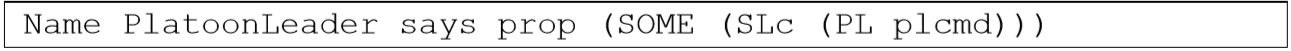
\includegraphics[width=0.7\linewidth]{name2.PNG}
\end{figure}

This input was a command from the \emph{PlatoonLeader}.  But, single commands of this type were not sufficient for more complex \emph{secure} state machines.  For more complex machines, several requests were required for a transition.  For example, in the ssmPlanPB secure state machine, to transition from the \emph{WARNO} state to the \emph{COMPLETE_PLAN} state, the machine had to pass through three other states first: \emph{TENTATIVE_PLAN, INITIATE_MOVEMENT}, and \emph{RECON}.  These three states were executed in any order.  But, all three had to be executed before transitioning to \emph{COMPLETE_PLAN}.  To do this, we transitioned directly from the \emph{WARNO} state to the \emph{COMPLETE_PLAN} state.  But, we changed the input for transition to be a list wherein the appropriate principals for each of the three non-sequential states and the \emph{WARNO} state had to issue the following commands:
  \begin{itemize}
  \item PlatoonLeader says tentativePlan,
   \item  PlatoonSergeant says initiateMovement, 
   \item PlatoonLeader says recon, 
   \item PlatoonLeader says completePlan
   \end{itemize}
   If all four commands were issued (and the principals were authorized), then HOL was instructed to allow the transition. \\
   
This type of list of multiple inputs allowed for the variation needed to represent the more complex \emph{secure} state machines in the project.  Of course, this type of input list was not permitted by ssm11.  The problem was in the description of the \emph{TR_rules, TR_cases, TR_ind}. The problem code was repeated in the blue text below in the following excerpt from \emph{TR_rules, TR_cases, TR_ind}.\\
     
\begin{figure}[h]
  \centering
  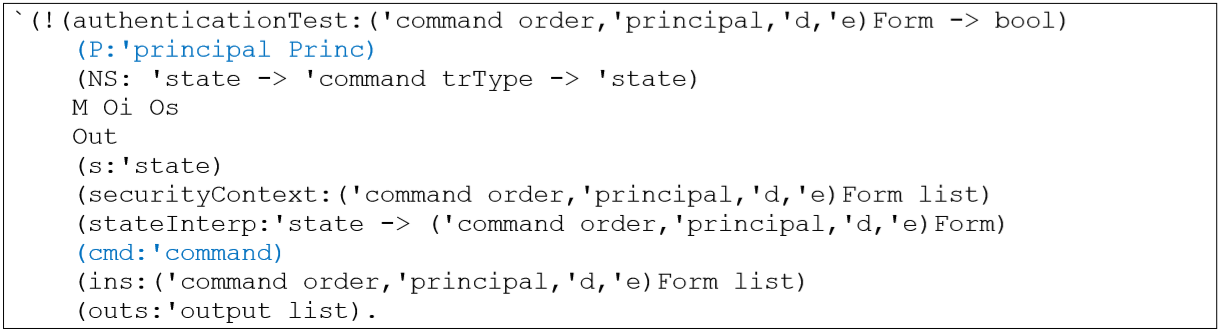
\includegraphics[width=0.8\linewidth]{authenticationTest.PNG}
\end{figure}

The code above was intended to be parameterized with the name of a principal and the type of command.  Then, HOL applied the pattern "Princ says command".  However, there were multiple principals with multiple commands and HOL required more information to accommodate this.  To accommodate this the Translation Relations had to be overhauled.  The accommodation required significant modification and verification of the code.  \\
  
  What follows explained where ssm differed from ssm11.

\subsubsection{Configurations}
\label{sec:configurations-2}

  Configurations did not change.

\subsubsection{Additional Functions}
\label{sec:additional-functions}

   Several additional functions were added to accommodate the overhaul. These functions are explained below.\\

   \begin{itemize}
   
   \item \underline{authenticationTest}\\
     \emph{authenticationTest} was not a new function.  But, its use was modified somewhat in ssm. The \emph{authenticationTest} function in ssm11 took an input stream as a parameter and returned true or false.  It was defined in each of the \emph{secure} state machines that parameterized ssm11.  The definition consisted of a conjunction of ACL formulas of the form "somePricnipal says someCommand = T".  The input stream was also of the same form needed by ssm11, in particular singleACLRequest::remainderOfList.  But, the input for ssm was not an input stream whose first element consisted of an ACL formula.  ssm's first element was a list of ACL formulas.  \\
      
    The \emph{authenticationTest} reduced the input list to a single T or F boolean value.  \emph{authenticationTest} took two parameters \emph{elementTest} followed by x.  \emph{elementTest} was a function and x was the input list.  \emph{elementTest} in ssm behaved exactly the same as \emph{authenticationTest} in ssm11.  \emph{elementTest} took a single ACL formula as input.  It returned true if the input was authenticated and false otherwise.  \emph{authenticationTest} in ssm did two things.  First, it mapped the \emph{elementTest} onto each element in the input list x. The result was a list of T or F boolean values.  \emph{authenticationTest} then "folded" the T boolean value onto this list.  The result in this case was T if all the elements in the list were true and false otherwise.  The code for \emph{authenticationTest} in ssm was shown below. \\
      
\begin{figure}[h]
  \centering
  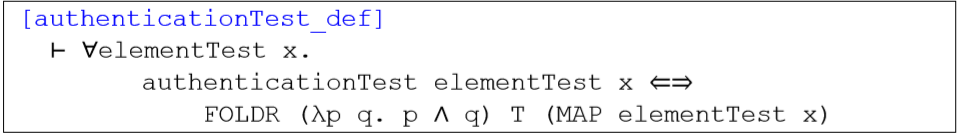
\includegraphics[width=0.6\linewidth]{authenticationTest2.PNG}
\end{figure}

 \item \underline{extractCommand}\\
 \emph{extractCommand} took an ACL request in the form of \emph{(P says prop (SOME cmd))} and extracted the command part of the request.  The definition for \emph{extractCommand} was shown below.\\
  
  \begin{figure}[h]
  \centering
  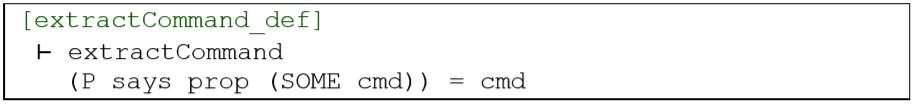
\includegraphics[width=0.6\linewidth]{extractCommand.PNG}
\end{figure}

 \item \underline{commandList}\\
\emph{commandList} mapped \emph{extractCommand} onto an input list.  The result was a list of commands.  The definition for the \emph{commandList} was shown below.\\
  
  \begin{figure}[h]
  \centering
  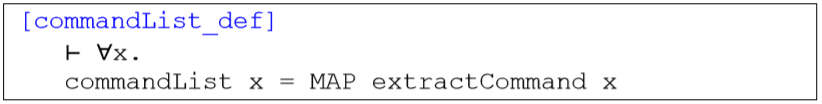
\includegraphics[width=0.6\linewidth]{commandList.PNG}
\end{figure}

 \item \underline{extractPropCommand}\\
   \emph{extractPropCommand} took an ACL request in the form of \emph{(P says prop (SOME cmd))} and extracted the proposition part of the request.  The definition for it was shown below.\\\\\\\\\\\\\\\\\\\\\\
   
  \begin{figure}[h]
  \centering
  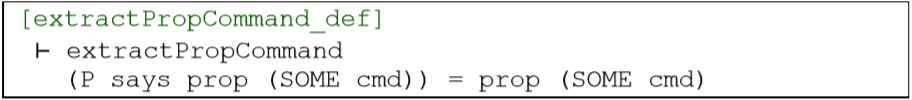
\includegraphics[width=0.6\linewidth]{extractPropCommand.PNG}
\end{figure}

\item \underline{propCommandList}\\
  \emph{propCommandList} mapped \emph{extractPropCommand} onto an input list.  The result was a list of propositions.  The definition for \emph{propCommandList} was shown below. \\
  
  \begin{figure}[h]
  \centering
  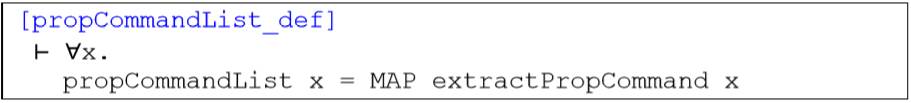
\includegraphics[width=0.6\linewidth]{propCommandList.PNG}
\end{figure}

 \item \underline{extractInput}\\
   \emph{extractInput} took an ACL formula of the form (P says prop x) and extracted the input x.  The definition for \emph{extractInput} was shown below.\\
   
  \begin{figure}[h]
  \centering
  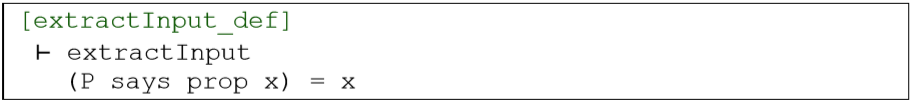
\includegraphics[width=0.6\linewidth]{extractInput.PNG}
\end{figure}

 \item \underline{inputList}\\
   \emph{inputList} mapped \emph{extractInput} onto an input list.  Thus, the result was a list of inputs.  The definition for \emph{inputList} was shown below.\\
   
  \begin{figure}[h!]
  \centering
  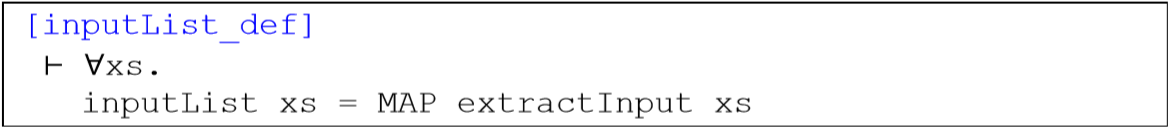
\includegraphics[width=0.6\linewidth]{inputList.PNG}
\end{figure}

 \item \underline{Theorems and Definitions}\\
 The remainder of the theorems and definitions in ssm were the same as those in ssm11.  Changes were made accommodate the different format of the input.  For the sake of brevity, they are not explained here.  The reader should view the EmitTeX pretty-printed files for ssm.
  \end{itemize}
 

  
\section{Secure State Machines Descriptions}
\label{sec:secure-state-mach}

\subsection{Top-level Secure State Machine}
\label{sec:top-level-secure}

This \emph{secure} state machine was named ssmPB and was also referred to as the top-level \emph{secure} state machine.  It used ssm11.  Figure 3.1 showed a diagram of the secure state machine.  The only principal for ssmPB was the Platoon Leader.   The six states allowed for a linear progression from the \emph{PLAN_PB} through \emph{MOVE_TO_ORP, CONDUCT_ORP, MOVE_TO_PB, CONDUCT_PB,} and finally to \emph{COMPLETE_PB}.  The \emph{incomplete} command allowed the secure state machine to remain at the same state.  Transition from the\emph{ PLAN_PB} state to \emph{MOVE_TO_ORP} state required the Platoon Leader issue the command \textbf{PlatoonLeader says \emph{crossLD}}.  Commands to transition to other states were self-naming: \emph{conductORP, moveToPB, conductPB,} and \emph{completePB}.\\\\\\\\

\begin{figure}[h]
  \centering
  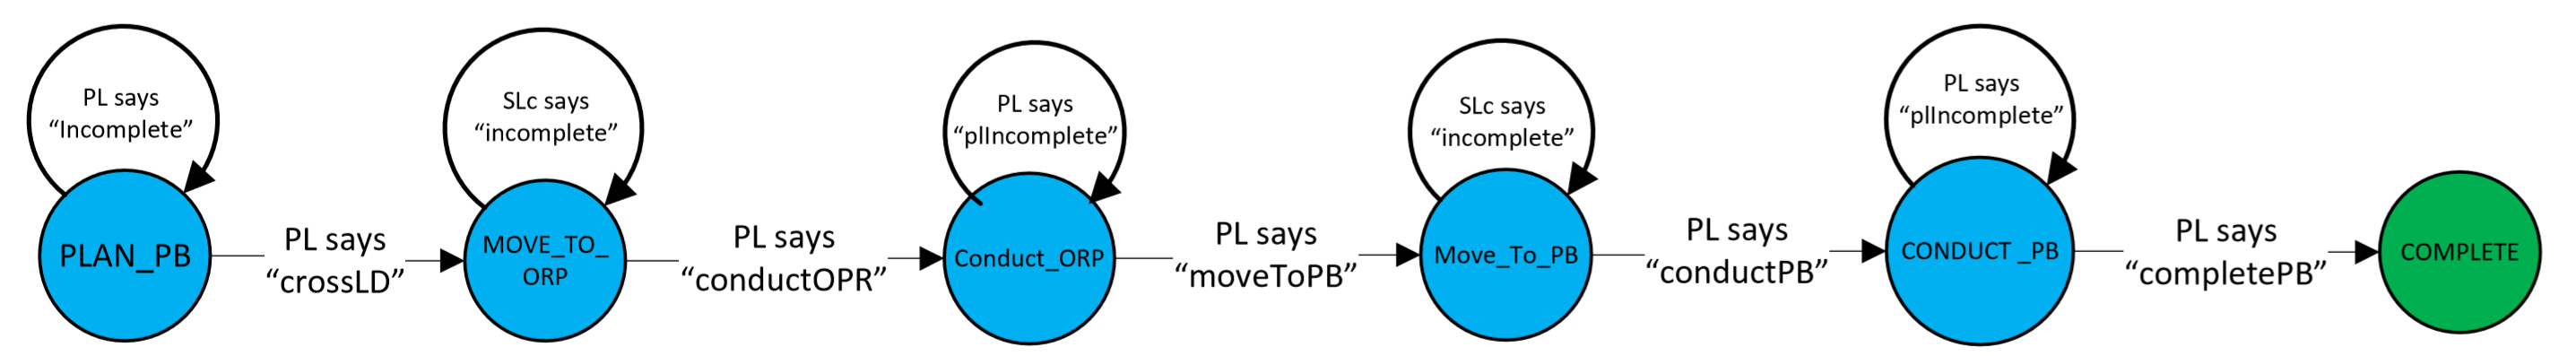
\includegraphics[width=1\linewidth]{diagram.PNG}
  \caption{Top-Level \emph{Secure} State Machine Diagram}
\end{figure}

The type file was saved in ABD/HOL/ssmPB/PBTypeScript.sml This file contained the datatype definitions and relevant theories for ssmPB.  The script file for the ssmPB theory was saved in ABD/HOL/ssmPB/ssmPBScript.sml.  This file contained the relevant theories to prove that transitions were justified if properly authenticated and authorized.

\subsection{Sub-level Secure State Machines}
\label{sec:sub-level-secure}

\underline{Planning Secure State Machine}
\begin{itemize}
\item Principals
\item States
\item Commands
\item Diagram
\item Difference with others
\end{itemize}


\subsubsection{Move To ORP Secure State Machine}
\label{sec:move-orp-secure}



This secure state machine was named ssmMoveToORP. It used ssm11.  Figure 3.2 showed a diagram of the secure state machine.  The only principal for ssmMoveToORP was the Platoon Leader.   The \emph{incomplete} command allowed the state machine to remain at the same state.  The state machine progressed sequentially from the \emph{MOVE_TO_ORP} state to \emph{PLT_FORM, PLT_MOVE, PLT_SECURE_HALT}, and finally to \emph{COMPLETE}.  The commands to transition among states were self-named: \emph{pltForm, pltMove, pltSecureHalt,} and \emph{complete}.  

\begin{figure}[h]
  \centering
  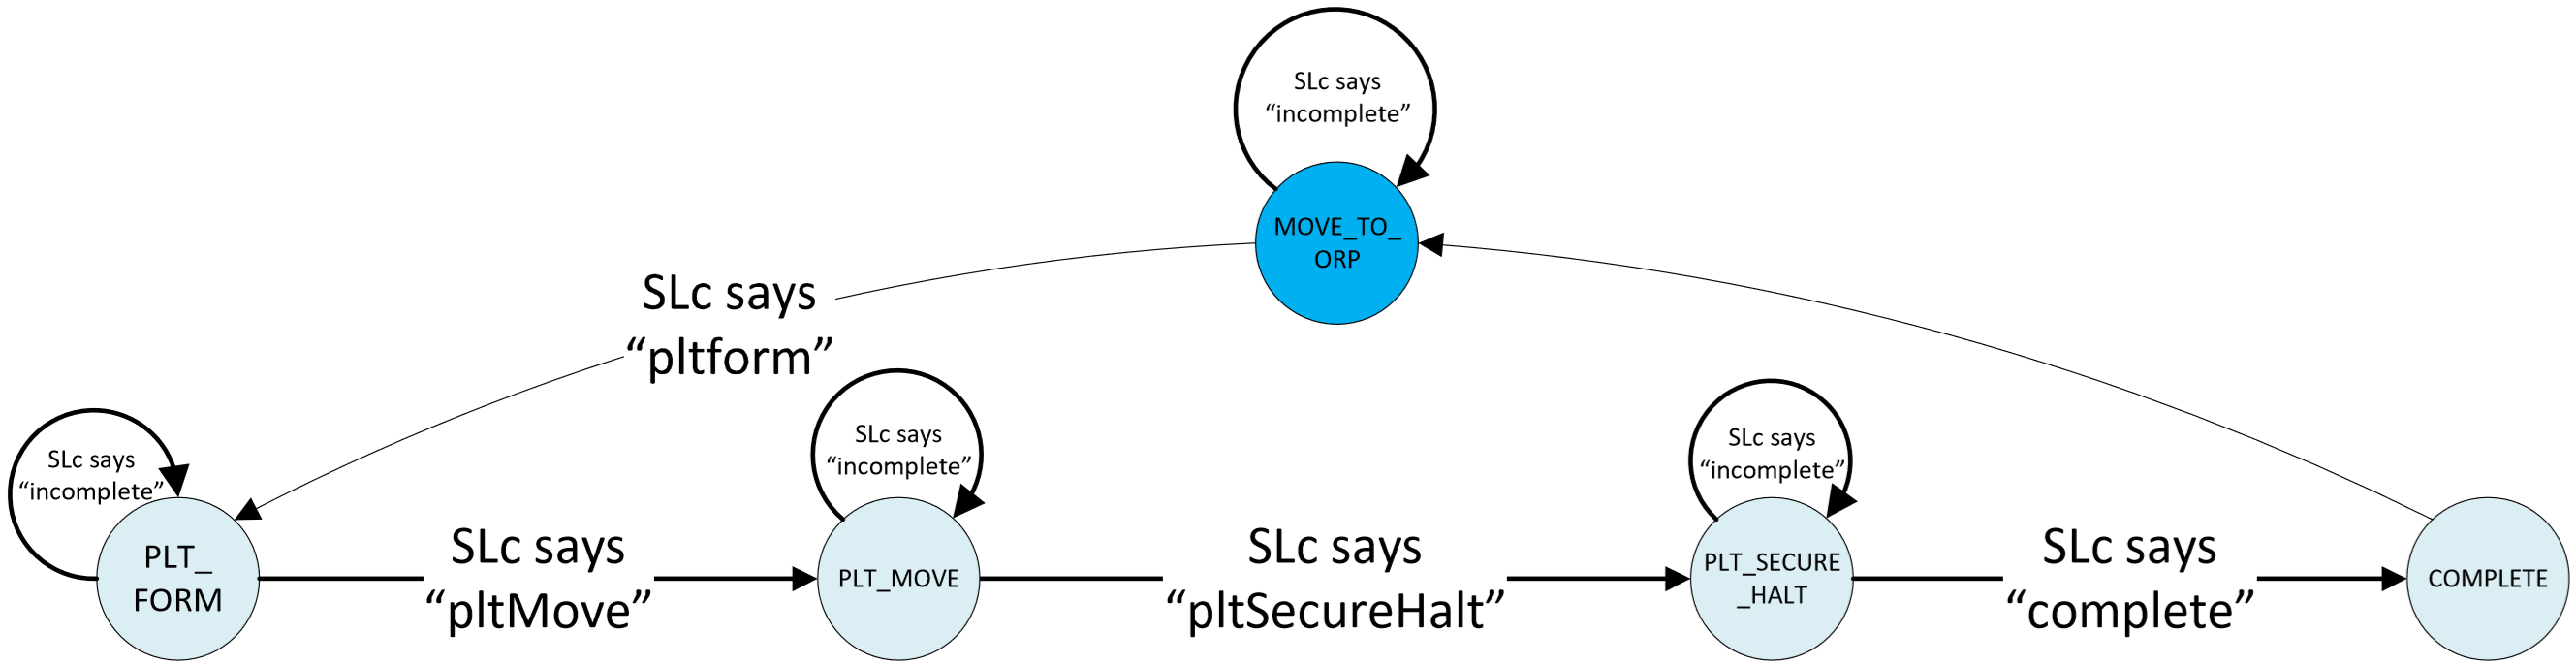
\includegraphics[width=1\linewidth]{MoveToORP.PNG}
  \caption{ssmMoveToORP \emph{Secure} State Machine Diagram}
\end{figure}

The type file was saved in ABD/HOL/ssmPB/subLevel/MoveToORPTypeScript.sml.  This file contained the datatype definitions and relevant theories for ssmMoveToORP.  The script file for the ssmMoveToORP theory was saved in ABD/HOL/ssmPB/subLevel/ssmMoveToORPScript.sml. This file contained the relevant theories to prove that transitions were justified if properly authenticated and authorized.

\subsubsection{Conduct ORP Secure State Machine}
\label{sec:conduct-orp-secure}

This \emph{secure} state machine was named ssmConductORP.  It used ssm11.  Figure 3.3 showed a diagram of the \emph{secure} state machine. There were two principals, Platoon Leader and Platoon Sergeant, with authorities on different states and transitions.  The Platoon Leader had authority to make state transitions on all states except for the \emph{SECURE} state.  The Platoon Sergeant only had authority to make a transition from the \emph{SECURE} state to the \emph{ACTIONS_IN} state or from the \emph{SECURE} state to itself.  The \emph{plIncomplete} and \emph{psgIncomplete} commands allowed the state machines to remain at the same state for the state in which that principal had authority.  The state machine progressed sequentially from the \emph{CONDUCT_ORP} state to\emph{ SECURE, ACTIONS_IN, WITHDRAW}, and finally \emph{COMPLETE}.   The commands to transition among states were self-named: \emph{secure, actionsIn, withdraw,} and \emph{complete}.

\begin{figure}[h]
  \centering
  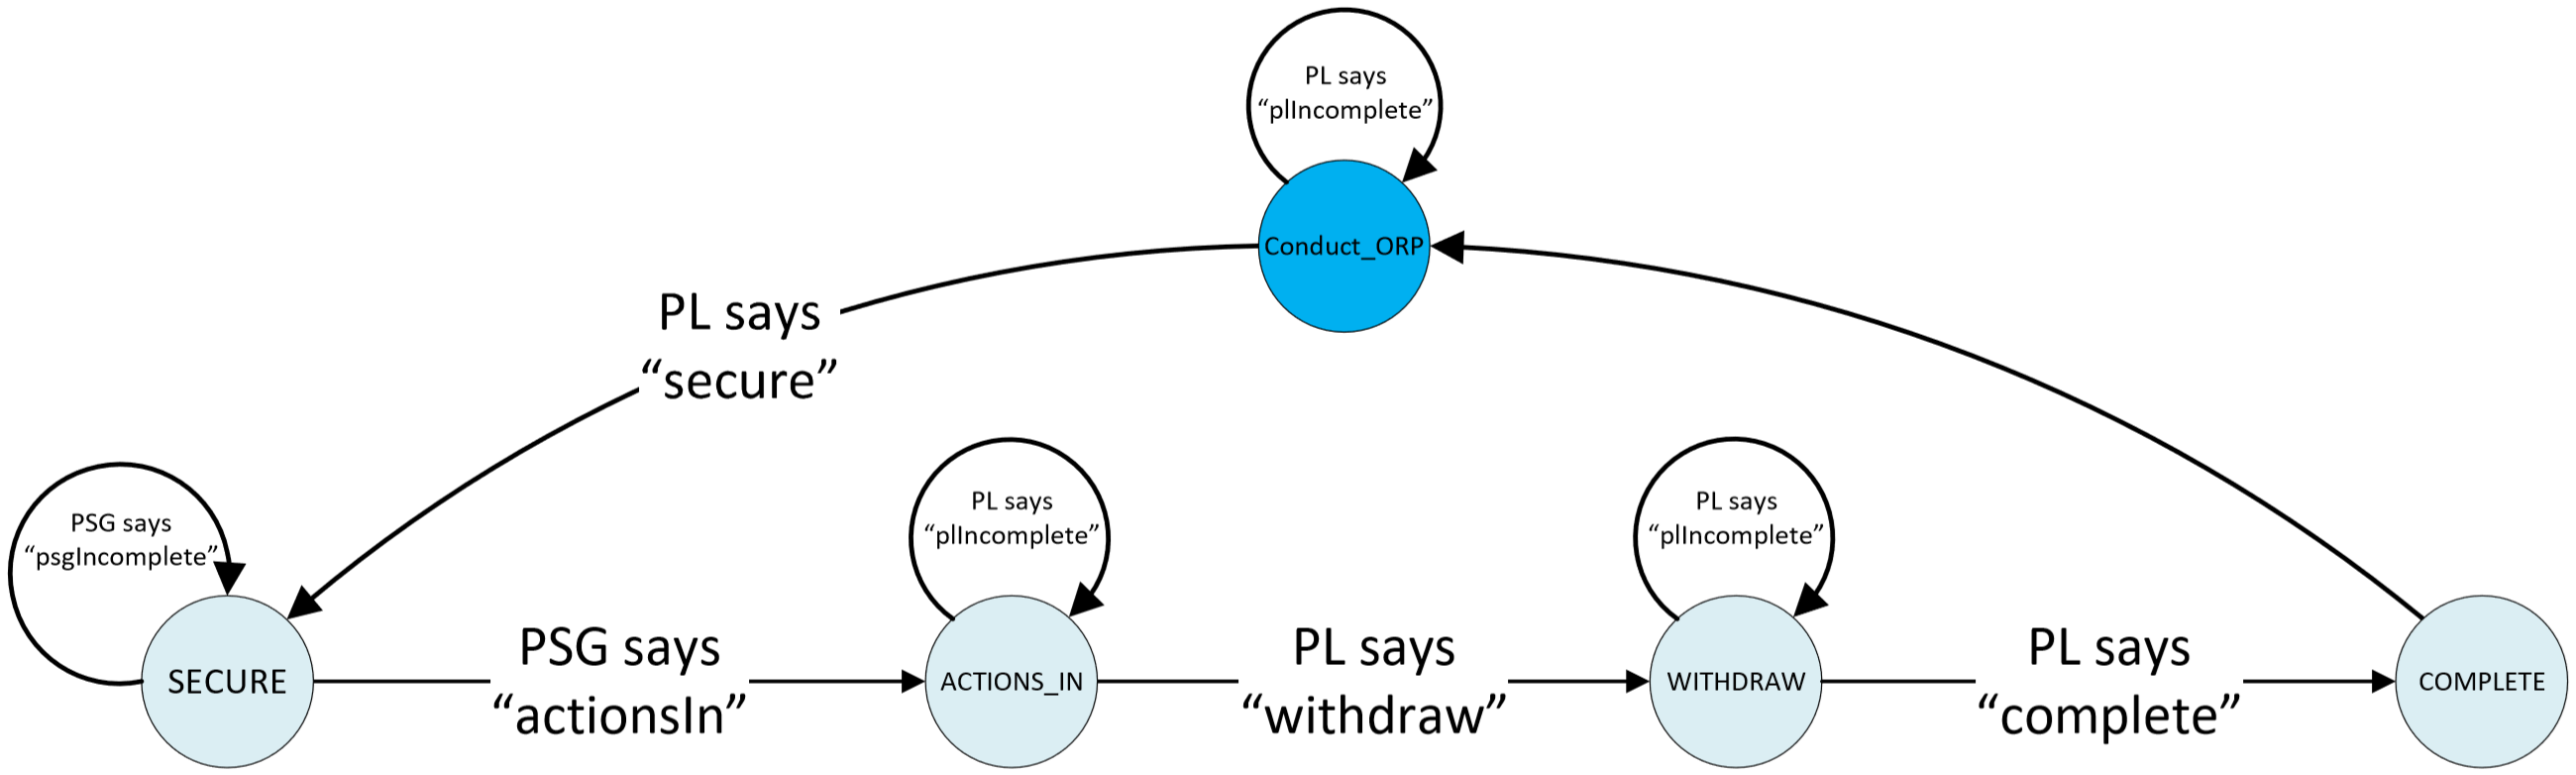
\includegraphics[width=1\linewidth]{ConductORP.PNG}
  \caption{ssmConductORP \emph{Secure} State Machine Diagram}
\end{figure}

The type file was saved in ABD/HOL/ssmPB/subLevel/ConductORPTypeScript.sml.  This file contained the datatype definitions and relevant theories for ssmConductORP.  The script file for the ssmConductORP theory was saved in ABD/HOL/ssmPB/subLevel/ssmConductORPScript.sml. This file contained the relevant theories to prove that transitions were justified if properly authenticated and authorized.


\subsubsection{Move To PB Secure State Machine}
\label{sec:move-pb-secure}

This \emph{secure} state machine was named ssmMoveToPB. It used ssm11.  Figure 3.4 showed a diagram of the secure state machine.  The only principal for ssmMoveToPB was the Platoon Leader.   The \emph{incomplete} command allowed the state machine to remain at the same state.  The state machine progressed sequentially from the \emph{MOVE_TO_PB} state to \emph{PLT_FORM, PLT_MOVE, PLT_HALT}, and finally to \emph{COMPLETE}.  The commands to transition among states were self-named: \emph{pltForm, pltMove, pltHalt,} and \emph{complete}.  \\\\\\\\\\\\\\\\\\\\\\\\\\\\\\

\begin{figure}[h]
  \centering
  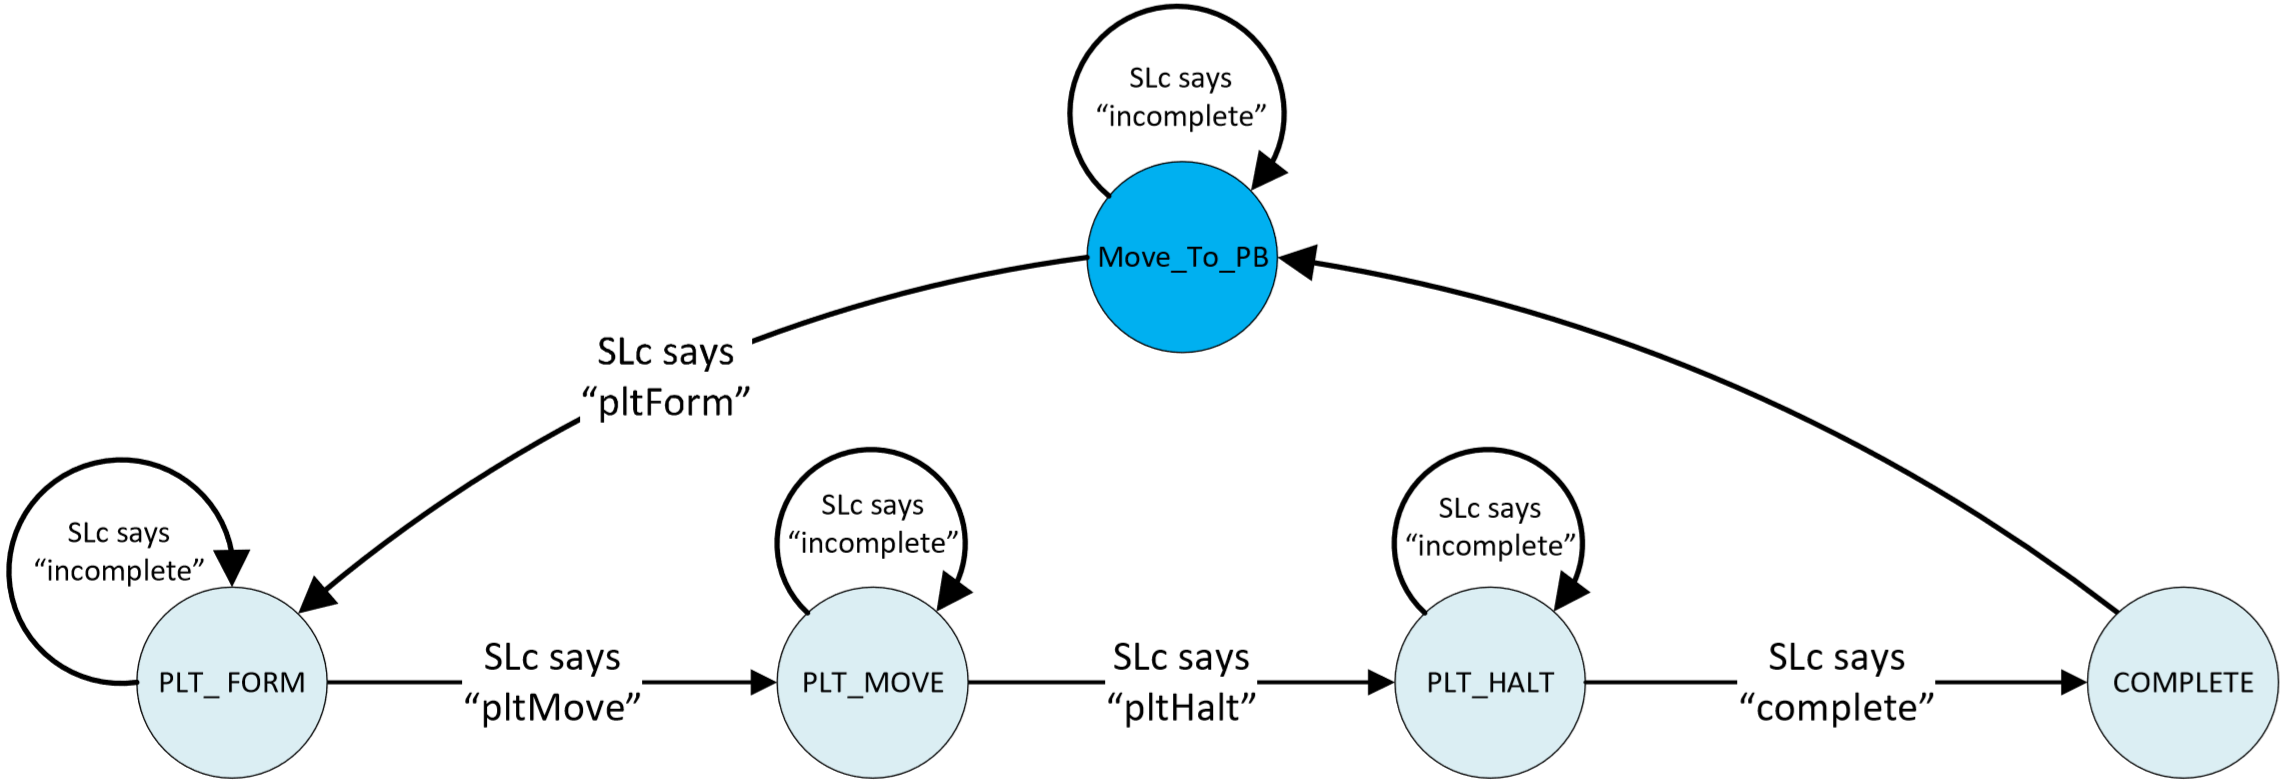
\includegraphics[width=1\linewidth]{MoveToPB2.PNG}
  \caption{ssmMoveToPB \emph{Secure} State Machine Diagram}
\end{figure}

The type file was saved in ABD/HOL/ssmPB/subLevel/MoveToPBTypeScript.sml.  This file contained the datatype definitions and relevant theories for ssmMoveToPB.  The script file for the ssmMoveToPB theory was saved in ABD/HOL/ssmPB/subLevel/ssmMoveToPBScript.sml. This file contained the relevant theories to prove that transitions were justified if properly authenticated and authorized.

\subsubsection{Conduct PB Secure State Machine}
\label{sec:conduct-pb-secure}

This \emph{secure} state machine was named ssmConductPB.  It used ssm11.  Figure 3.5 showed a diagram of the secure state machine. There were two principals, Platoon Leader and Platoon Sergeant, with authorities on different states and transitions.  The Platoon Leader had authority to make state transitions on all states except for the \emph{SECURE_PB} state.  The Platoon Sergeant only had authority to make a transition from the \emph{SECURE_PB} state to the \emph{ACTIONS_IN_PB} state or from the \emph{SECURE} state to itself.  The \emph{plIncompletePB} and \emph{psgIncompletePB} commands allowed the state machines to remain at the same state for the state in which that principal had authority.  The state machine progressed sequentially from the \emph{CONDUCT_PB} state to \emph{SECURE, ACTIONS_IN_PB, WITHDRAW_PB}, and finally \emph{COMPLETE_PB}.   The commands to transition among states were self-named: \emph{securePB, actionsInPB, withdrawPB,} and \emph{completePB}.

\begin{figure}[h]
  \centering
  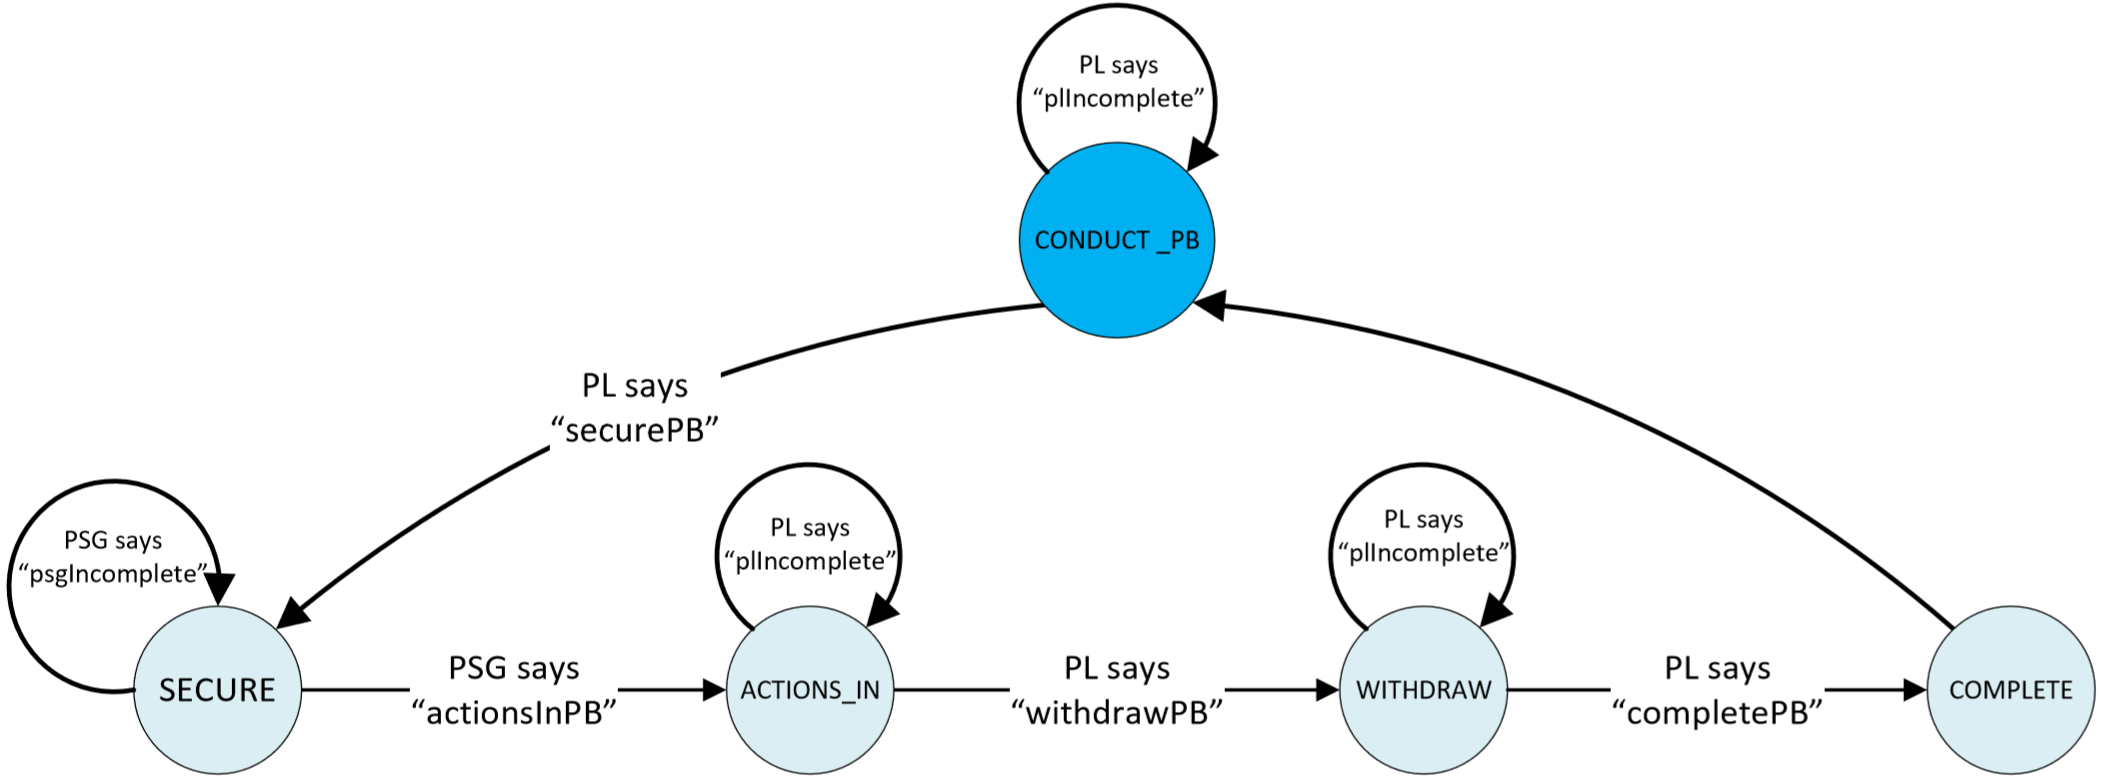
\includegraphics[width=1\linewidth]{ConductPB.PNG}
  \caption{ssmConductPB \emph{Secure} State Machine Diagram}
\end{figure}

The type file was saved in ABD/HOL/ssmPB/subLevel/ConductPBTypeScript.sml.  This file contained the datatype definitions and relevant theories for ssmConductPB.  The script file for the ssmConductPB theory was saved in ABD/HOL/ssmPB/subLevel/ssmConductPBScript.sml. This file contained the relevant theories to prove that transitions were justified if properly authenticated and authorized.

\subsection{Sub-sub-level Secure State Machines}
\label{sec:sub-sub-level-1}

The sub-sub-level \emph{secure} state machines were reserved for future work at the time of this documentation.  These \emph{secure} state machines require more complexity because they were at a lower level of abstraction.  The added complexity required the overhaul of the ssm11 to smm.  Nevertheless, these \emph{secure} state machines were discussed in detail and ready to be verified in HOL.

\subsection{Other Structures}
\label{sec:other-structures}

In addition to the levels of state machines, additional theories were discussed and planned for future work.  A platoon theory, squad theory, and soldier theory was discussed.  They wre discussed in the Future Work section at the time of this documentation.


% ---- this points LaTeX to PatrolBaseDoc.tex ----
% Local Variables:
% TeX-master: "../PatrolBaseDoc"
% End: